% Options for packages loaded elsewhere
\PassOptionsToPackage{unicode}{hyperref}
\PassOptionsToPackage{hyphens}{url}
\PassOptionsToPackage{dvipsnames,svgnames*,x11names*}{xcolor}
%
\documentclass[
  10pt,
]{article}
\usepackage{amsmath,amssymb}
\usepackage{lmodern}
\usepackage{ifxetex,ifluatex}
\ifnum 0\ifxetex 1\fi\ifluatex 1\fi=0 % if pdftex
  \usepackage[T1]{fontenc}
  \usepackage[utf8]{inputenc}
  \usepackage{textcomp} % provide euro and other symbols
\else % if luatex or xetex
  \usepackage{unicode-math}
  \defaultfontfeatures{Scale=MatchLowercase}
  \defaultfontfeatures[\rmfamily]{Ligatures=TeX,Scale=1}
\fi
% Use upquote if available, for straight quotes in verbatim environments
\IfFileExists{upquote.sty}{\usepackage{upquote}}{}
\IfFileExists{microtype.sty}{% use microtype if available
  \usepackage[]{microtype}
  \UseMicrotypeSet[protrusion]{basicmath} % disable protrusion for tt fonts
}{}
\makeatletter
\@ifundefined{KOMAClassName}{% if non-KOMA class
  \IfFileExists{parskip.sty}{%
    \usepackage{parskip}
  }{% else
    \setlength{\parindent}{0pt}
    \setlength{\parskip}{6pt plus 2pt minus 1pt}}
}{% if KOMA class
  \KOMAoptions{parskip=half}}
\makeatother
\usepackage{xcolor}
\IfFileExists{xurl.sty}{\usepackage{xurl}}{} % add URL line breaks if available
\IfFileExists{bookmark.sty}{\usepackage{bookmark}}{\usepackage{hyperref}}
\hypersetup{
  pdftitle={Using R tools for analysis  of primary biodiversity data provided by SBDI},
  pdfauthor={Debora Arlt and Alejandro Ruete  for the Swedish Biodiversity Data Infrastructure},
  colorlinks=true,
  linkcolor=Maroon,
  filecolor=Maroon,
  citecolor=Blue,
  urlcolor=Blue,
  pdfcreator={LaTeX via pandoc}}
\urlstyle{same} % disable monospaced font for URLs
\usepackage[margin=1in]{geometry}
\usepackage{color}
\usepackage{fancyvrb}
\newcommand{\VerbBar}{|}
\newcommand{\VERB}{\Verb[commandchars=\\\{\}]}
\DefineVerbatimEnvironment{Highlighting}{Verbatim}{commandchars=\\\{\}}
% Add ',fontsize=\small' for more characters per line
\usepackage{framed}
\definecolor{shadecolor}{RGB}{248,248,248}
\newenvironment{Shaded}{\begin{snugshade}}{\end{snugshade}}
\newcommand{\AlertTok}[1]{\textcolor[rgb]{0.94,0.16,0.16}{#1}}
\newcommand{\AnnotationTok}[1]{\textcolor[rgb]{0.56,0.35,0.01}{\textbf{\textit{#1}}}}
\newcommand{\AttributeTok}[1]{\textcolor[rgb]{0.77,0.63,0.00}{#1}}
\newcommand{\BaseNTok}[1]{\textcolor[rgb]{0.00,0.00,0.81}{#1}}
\newcommand{\BuiltInTok}[1]{#1}
\newcommand{\CharTok}[1]{\textcolor[rgb]{0.31,0.60,0.02}{#1}}
\newcommand{\CommentTok}[1]{\textcolor[rgb]{0.56,0.35,0.01}{\textit{#1}}}
\newcommand{\CommentVarTok}[1]{\textcolor[rgb]{0.56,0.35,0.01}{\textbf{\textit{#1}}}}
\newcommand{\ConstantTok}[1]{\textcolor[rgb]{0.00,0.00,0.00}{#1}}
\newcommand{\ControlFlowTok}[1]{\textcolor[rgb]{0.13,0.29,0.53}{\textbf{#1}}}
\newcommand{\DataTypeTok}[1]{\textcolor[rgb]{0.13,0.29,0.53}{#1}}
\newcommand{\DecValTok}[1]{\textcolor[rgb]{0.00,0.00,0.81}{#1}}
\newcommand{\DocumentationTok}[1]{\textcolor[rgb]{0.56,0.35,0.01}{\textbf{\textit{#1}}}}
\newcommand{\ErrorTok}[1]{\textcolor[rgb]{0.64,0.00,0.00}{\textbf{#1}}}
\newcommand{\ExtensionTok}[1]{#1}
\newcommand{\FloatTok}[1]{\textcolor[rgb]{0.00,0.00,0.81}{#1}}
\newcommand{\FunctionTok}[1]{\textcolor[rgb]{0.00,0.00,0.00}{#1}}
\newcommand{\ImportTok}[1]{#1}
\newcommand{\InformationTok}[1]{\textcolor[rgb]{0.56,0.35,0.01}{\textbf{\textit{#1}}}}
\newcommand{\KeywordTok}[1]{\textcolor[rgb]{0.13,0.29,0.53}{\textbf{#1}}}
\newcommand{\NormalTok}[1]{#1}
\newcommand{\OperatorTok}[1]{\textcolor[rgb]{0.81,0.36,0.00}{\textbf{#1}}}
\newcommand{\OtherTok}[1]{\textcolor[rgb]{0.56,0.35,0.01}{#1}}
\newcommand{\PreprocessorTok}[1]{\textcolor[rgb]{0.56,0.35,0.01}{\textit{#1}}}
\newcommand{\RegionMarkerTok}[1]{#1}
\newcommand{\SpecialCharTok}[1]{\textcolor[rgb]{0.00,0.00,0.00}{#1}}
\newcommand{\SpecialStringTok}[1]{\textcolor[rgb]{0.31,0.60,0.02}{#1}}
\newcommand{\StringTok}[1]{\textcolor[rgb]{0.31,0.60,0.02}{#1}}
\newcommand{\VariableTok}[1]{\textcolor[rgb]{0.00,0.00,0.00}{#1}}
\newcommand{\VerbatimStringTok}[1]{\textcolor[rgb]{0.31,0.60,0.02}{#1}}
\newcommand{\WarningTok}[1]{\textcolor[rgb]{0.56,0.35,0.01}{\textbf{\textit{#1}}}}
\usepackage{longtable,booktabs,array}
\usepackage{calc} % for calculating minipage widths
% Correct order of tables after \paragraph or \subparagraph
\usepackage{etoolbox}
\makeatletter
\patchcmd\longtable{\par}{\if@noskipsec\mbox{}\fi\par}{}{}
\makeatother
% Allow footnotes in longtable head/foot
\IfFileExists{footnotehyper.sty}{\usepackage{footnotehyper}}{\usepackage{footnote}}
\makesavenoteenv{longtable}
\usepackage{graphicx}
\makeatletter
\def\maxwidth{\ifdim\Gin@nat@width>\linewidth\linewidth\else\Gin@nat@width\fi}
\def\maxheight{\ifdim\Gin@nat@height>\textheight\textheight\else\Gin@nat@height\fi}
\makeatother
% Scale images if necessary, so that they will not overflow the page
% margins by default, and it is still possible to overwrite the defaults
% using explicit options in \includegraphics[width, height, ...]{}
\setkeys{Gin}{width=\maxwidth,height=\maxheight,keepaspectratio}
% Set default figure placement to htbp
\makeatletter
\def\fps@figure{htbp}
\makeatother
\setlength{\emergencystretch}{3em} % prevent overfull lines
\providecommand{\tightlist}{%
  \setlength{\itemsep}{0pt}\setlength{\parskip}{0pt}}
\setcounter{secnumdepth}{5}
\ifluatex
  \usepackage{selnolig}  % disable illegal ligatures
\fi
\usepackage[]{natbib}
\bibliographystyle{apalike}

\title{Using R tools for analysis of primary biodiversity data provided by SBDI}
\author{Debora Arlt and Alejandro Ruete for the Swedish Biodiversity Data Infrastructure}
\date{2021-10-05}

\begin{document}
\maketitle

{
\hypersetup{linkcolor=}
\setcounter{tocdepth}{2}
\tableofcontents
}
\hypertarget{introduction}{%
\section*{Introduction}\label{introduction}}
\addcontentsline{toc}{section}{Introduction}

Biodiversity resources are increasingly international. The SBDI has made an effort to canalise biodiversity data and resources to help the research community access and analyse Swedish primary biodiversity data. Each research question draws its own challenges which are unique in themselves. Our aim here is to provide a few examples that prompt questions that may be asked at different stages of the process. The validity and appropriateness of a particular method depends on the individual researcher(s). For a comprehensive workflow on how to treat and analyse primary biodiversity data please refer to our tutorial on \href{https://github.com/biodiversitydata-se/biodiversity-analysis-tools}{biodiversity analysis tools} where we go through the complete workflow Data --\textgreater{} Cleaning --\textgreater{} Fitness evaluation --\textgreater{} Analysis

\hypertarget{r-and-mirroreum}{%
\subsection*{R and Mirroreum}\label{r-and-mirroreum}}
\addcontentsline{toc}{subsection}{R and Mirroreum}

The present tutorial is focused on the statistical programming language R. R is a free software environment for statistical computing and graphics that is widely used within the scientific community and where the complete analysis workflow can be documented in a fully reproducible way.

At SBDI we provide access for researchers and students to \href{https://mirroreum.biodiversitydata.se/}{Mirroreum} -- an online web-based environment for Reproducible Open Research in the area of biodiversity analysis. Mirroreum is based on a Free and Open Source stack of software. Logging in, you immediately get access to a web-based version of R Studio with a large number of pre-installed packages such as all the packages offered from ROpenSci and more.

Compared to running R Studio on your own machine, Mirroreum offers more computational resources and a standardized environment where you can rely on all the relevant packages being installed and the configuration parameters being set appropriately. To know more about Mirroreum or to request an account please visit the \href{https://docs.biodiversitydata.se/analyse-data/mirroreum/}{SBDI documentation site}

\href{https://mirroreum.biodiversitydata.se/auth-sign-in}{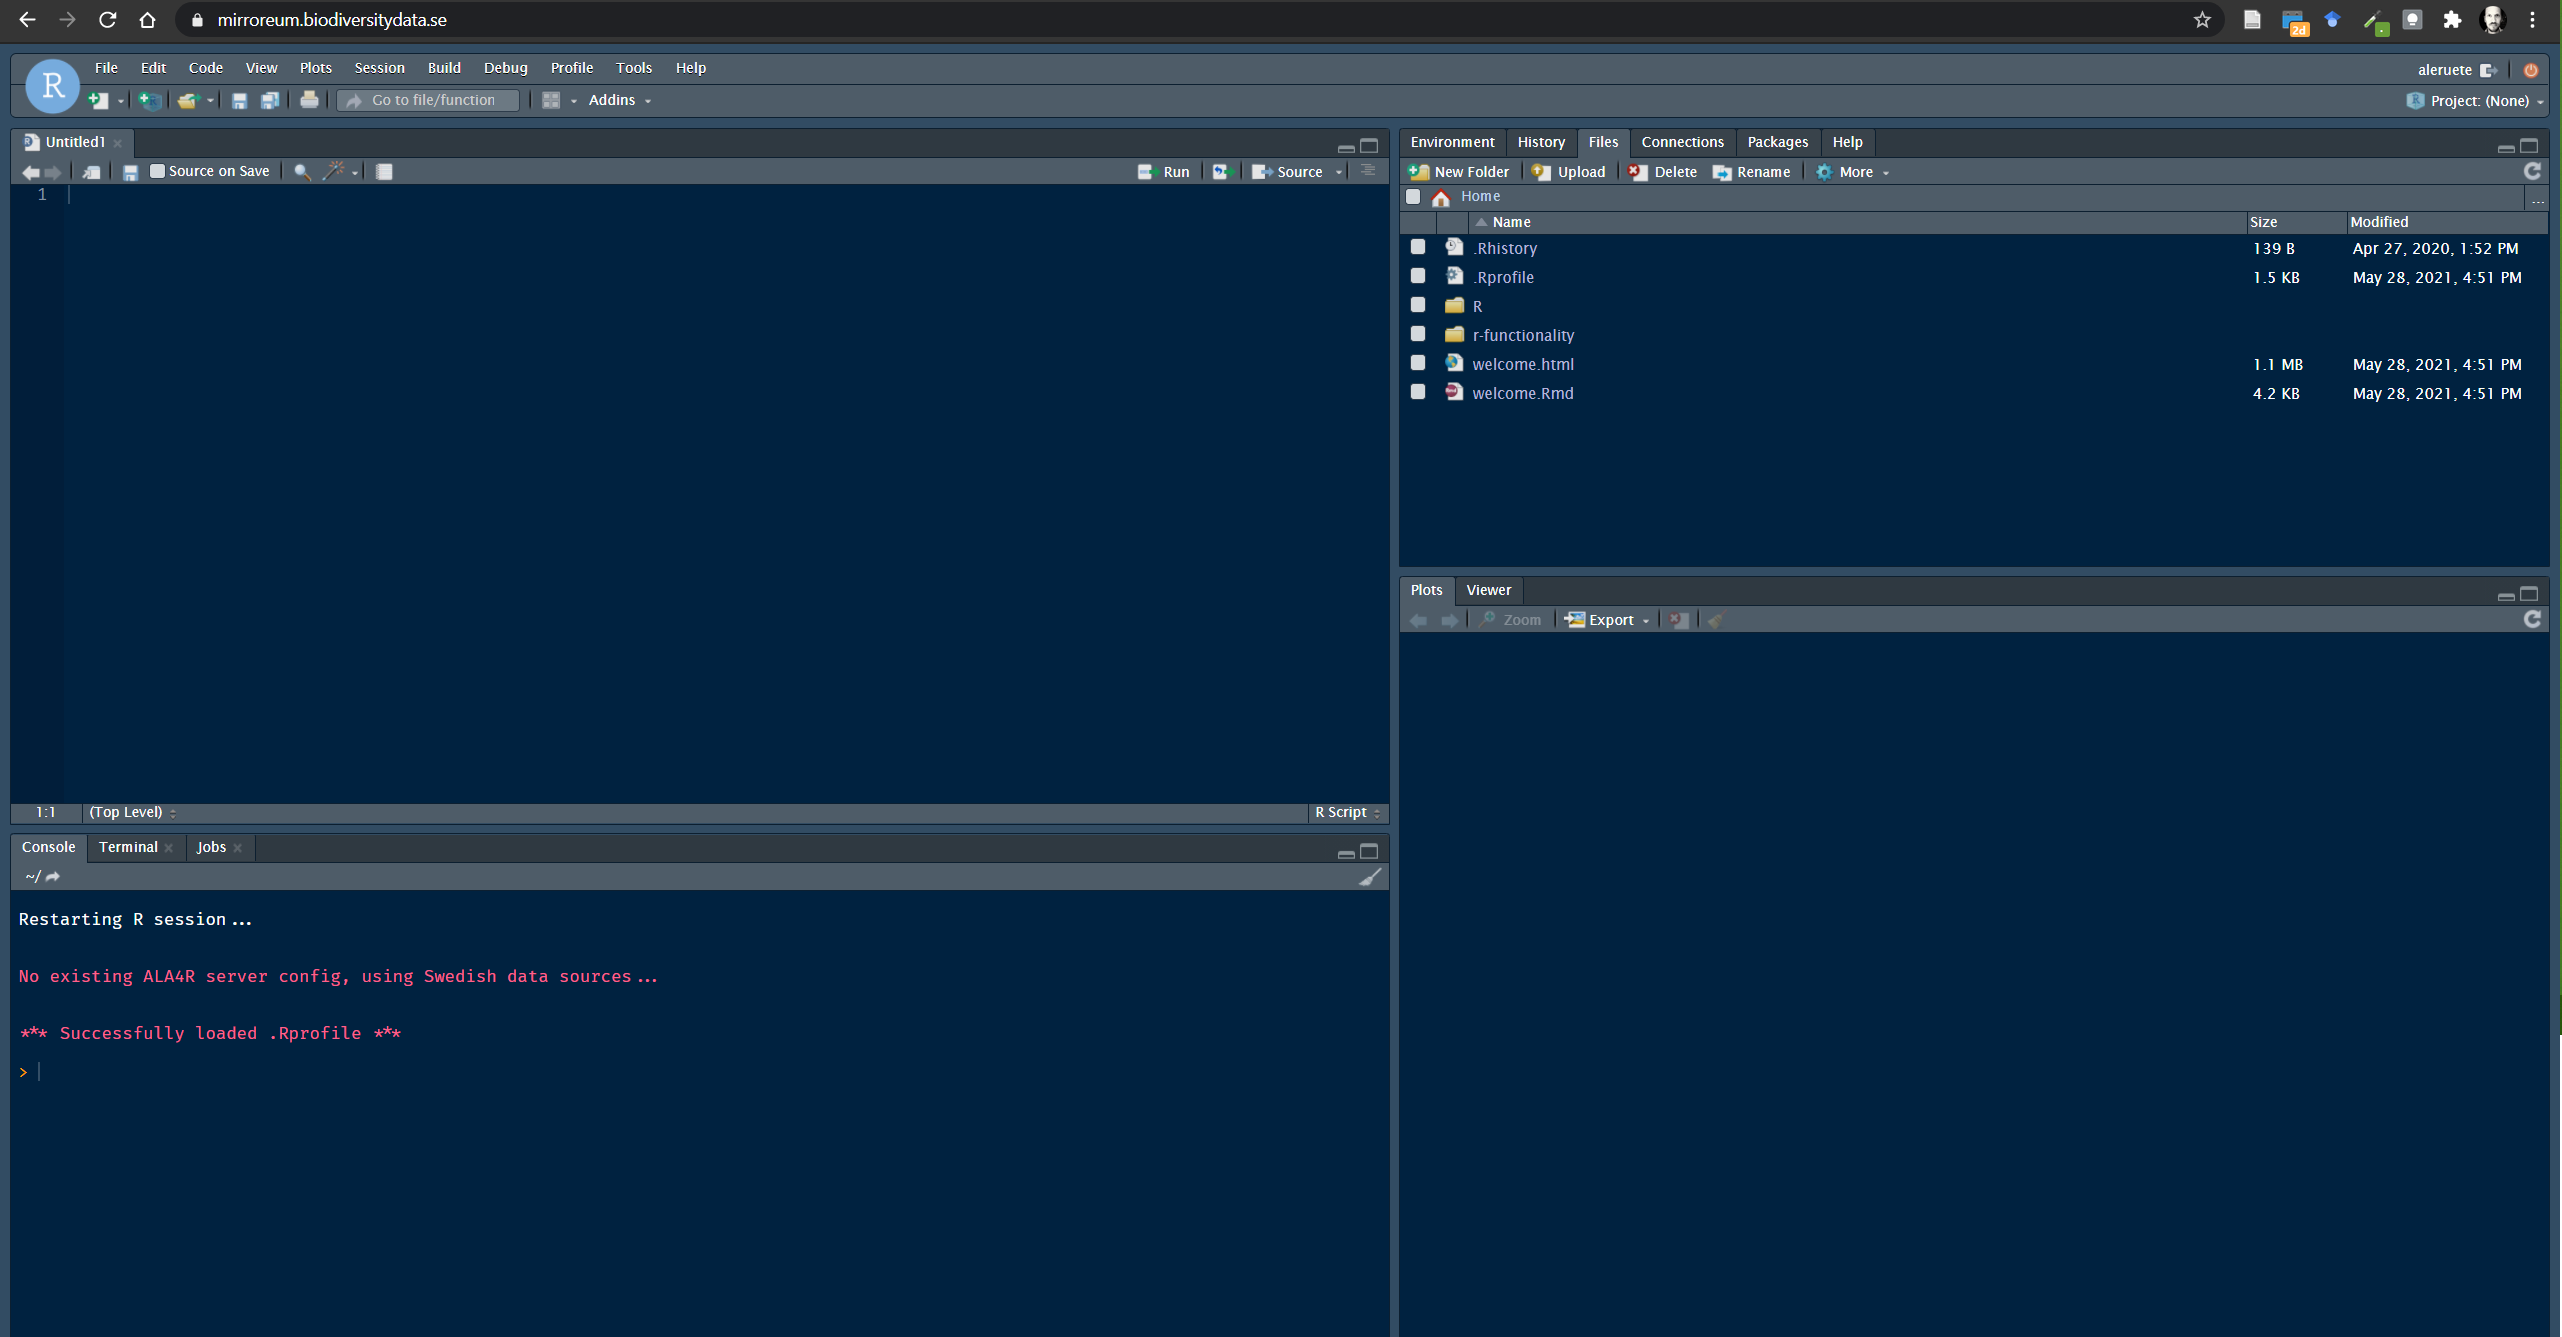
\includegraphics{images/Mirroreum.png}}

\hypertarget{sbdi4r---an-r-to-search-an-access-data}{%
\subsection*{SBDI4R - an R 📦 to search an access data}\label{sbdi4r---an-r-to-search-an-access-data}}
\addcontentsline{toc}{subsection}{SBDI4R - an R 📦 to search an access data}

The SBDI4R package enables the R community to directly access data and resources hosted by SBDI. The goal is to enable observations of species to be queried and output in a range of standard formats. It includes some filter functions that allow you to filter prior to download. It also includes some simple summary functions, and some function for some simple data exploration. The examples included in this tutorial also show you how you can continue exploring and analyzing using other R package.

Please refer to the \href{https://biodiversitydata-se.github.io/SBDI4R}{package documentation} for details on how to install it. Once installed the SBDI4R package must be loaded for each new R session:

\begin{Shaded}
\begin{Highlighting}[]
\FunctionTok{library}\NormalTok{(SBDI4R)}
\end{Highlighting}
\end{Shaded}

Various aspects of the SBDI4R package can be customized.

\hypertarget{caching}{%
\paragraph*{Caching}\label{caching}}
\addcontentsline{toc}{paragraph}{Caching}

SBDI4R can cache most results to local files. This means that if the same code is run multiple times, the second and subsequent iterations will be faster. This will also reduce load on the web servers. By default, this caching is session-based, meaning that the local files are stored in a temporary directory that is automatically deleted when the R session is ended. This behavior can be altered so that caching is permanent, by setting the caching directory to a non-temporary location. For example, under Windows, use something like:

\begin{Shaded}
\begin{Highlighting}[]
\FunctionTok{sbdi\_config}\NormalTok{(}\AttributeTok{cache\_directory =} \FunctionTok{file.path}\NormalTok{(}\StringTok{"c:"}\NormalTok{,}\StringTok{"mydata"}\NormalTok{,}\StringTok{"sbdi\_cache"}\NormalTok{)) }\DocumentationTok{\#\# Windows}
\end{Highlighting}
\end{Shaded}

or for Linux:

\begin{Shaded}
\begin{Highlighting}[]
\FunctionTok{sbdi\_config}\NormalTok{(}\AttributeTok{cache\_directory =} \StringTok{"\textasciitilde{}/mydata/sbdi\_cache"}\NormalTok{) }\DocumentationTok{\#\# Linux}
\end{Highlighting}
\end{Shaded}

Note that this directory must exist (you need to create it yourself).

All results will be stored in that cache directory and will be used from one session to the next. They won't be re-downloaded from the server unless the user specifically deletes those files or changes the caching setting to ``refresh''.

If you change the cache\_directory to a permanent location, you may wish to add something like this to your .Rprofile file, so that it happens automatically each time the SBDI4R package is loaded:

\begin{Shaded}
\begin{Highlighting}[]
\FunctionTok{setHook}\NormalTok{(}\FunctionTok{packageEvent}\NormalTok{(}\StringTok{"SBDI4R"}\NormalTok{, }\StringTok{"onLoad"}\NormalTok{), }
        \ControlFlowTok{function}\NormalTok{(...) }\FunctionTok{sbdi\_config}\NormalTok{(}\AttributeTok{cache\_directory=}\FunctionTok{file.path}\NormalTok{(}\StringTok{"\textasciitilde{}"}\NormalTok{,}\StringTok{"mydata"}\NormalTok{,}\StringTok{"sbdi\_cache"}\NormalTok{)))}
\end{Highlighting}
\end{Shaded}

Caching can also be turned off entirely by:

\begin{Shaded}
\begin{Highlighting}[]
\FunctionTok{sbdi\_config}\NormalTok{(}\AttributeTok{caching=}\StringTok{"off"}\NormalTok{)}
\end{Highlighting}
\end{Shaded}

or set to ``refresh'', meaning that the cached results will re-downloaded from the SBDI servers and the cache updated. (This will happen for as long as caching is set to ``refresh'' --- so you may wish to switch back to normal ``on'' caching behavior once you have updated your cache with the data you are working on).

\hypertarget{e-mail-address}{%
\paragraph*{E-mail address}\label{e-mail-address}}
\addcontentsline{toc}{paragraph}{E-mail address}

Each download request to SBDI servers is also accompanied by an ``e-mail address'' string that identifies the user making the request. You will need to provide an email address registered with the SBDI. You can create an account \href{https://auth.biodiversitydata.se/cas/login}{here}. Once an email is registered with the SBDI, it should be stored in the config:

\begin{Shaded}
\begin{Highlighting}[]
\FunctionTok{sbdi\_config}\NormalTok{(}\AttributeTok{email=}\StringTok{"your.valid@emailaddress.com"}\NormalTok{)}
\end{Highlighting}
\end{Shaded}

Else you can provide this e-mail address as a parameter directly to each call of the function occurrences().

\hypertarget{setting-the-download-reason}{%
\paragraph*{Setting the download reason}\label{setting-the-download-reason}}
\addcontentsline{toc}{paragraph}{Setting the download reason}

SBDI requires that you provide a reason when downloading occurrence data (via the SBDI4R \texttt{occurrences()} function). You can provide this as a parameter directly to each call of \texttt{occurrences()}, or you can set it once per session using:

\begin{Shaded}
\begin{Highlighting}[]
\FunctionTok{sbdi\_config}\NormalTok{(}\AttributeTok{download\_reason\_id =} \StringTok{"your\_reason\_id"}\NormalTok{)}
\end{Highlighting}
\end{Shaded}

(See \texttt{sbdi\_reasons()} for valid download reasons, e.g.~* 3 for ``education'', * 7 for ``ecological research'', * 8 for ``systematic research/taxonomy'', * 10 for ``testing'')

\hypertarget{privacy}{%
\paragraph*{Privacy}\label{privacy}}
\addcontentsline{toc}{paragraph}{Privacy}

\textbf{\emph{NO}} other personal identification information is sent. You can see all configuration settings, including the the user-agent string that is being used, with the command:

\begin{Shaded}
\begin{Highlighting}[]
\FunctionTok{sbdi\_config}\NormalTok{()}
\end{Highlighting}
\end{Shaded}

\hypertarget{other-options}{%
\paragraph*{Other options}\label{other-options}}
\addcontentsline{toc}{paragraph}{Other options}

If you make a request that returns an empty result set (e.g.~an un-matched name), by default you will simply get an empty data structure returned to you without any special notification. If you would like to be warned about empty result sets, you can use:

\begin{Shaded}
\begin{Highlighting}[]
\FunctionTok{sbdi\_config}\NormalTok{(}\AttributeTok{warn\_on\_empty=}\ConstantTok{TRUE}\NormalTok{)}
\end{Highlighting}
\end{Shaded}

\hypertarget{other-packages-needed}{%
\subsection*{Other packages needed}\label{other-packages-needed}}
\addcontentsline{toc}{subsection}{Other packages needed}

Some additional packages are needed for these examples. Install them if necessary with the following script:

\begin{Shaded}
\begin{Highlighting}[]
\NormalTok{to\_install }\OtherTok{\textless{}{-}} \FunctionTok{c}\NormalTok{(}\StringTok{"colorRamps"}\NormalTok{, }\StringTok{"cowplot"}\NormalTok{,}\StringTok{"dplyr"}\NormalTok{,}\StringTok{"ggplot2"}\NormalTok{, }
                \StringTok{"leaflet"}\NormalTok{, }\StringTok{"maps"}\NormalTok{, }\StringTok{"mapdata"}\NormalTok{, }\StringTok{"maptools"}\NormalTok{, }\StringTok{"sf"}\NormalTok{, }
                \StringTok{"remotes"}\NormalTok{,}\StringTok{"rgeos"}\NormalTok{,}\StringTok{"tidyr"}\NormalTok{, }\StringTok{"xts"}\NormalTok{)}
\NormalTok{to\_install }\OtherTok{\textless{}{-}}\NormalTok{ to\_install[}\SpecialCharTok{!}\FunctionTok{sapply}\NormalTok{(to\_install, }
\NormalTok{                                 requireNamespace, }
                                 \AttributeTok{quietly=}\ConstantTok{TRUE}\NormalTok{)]}
\ControlFlowTok{if}\NormalTok{(}\FunctionTok{length}\NormalTok{(to\_install)}\SpecialCharTok{\textgreater{}}\DecValTok{0}\NormalTok{)}
    \FunctionTok{install.packages}\NormalTok{(to\_install, }
                     \AttributeTok{repos=}\StringTok{"http://cran.us.r{-}project.org"}\NormalTok{)}

\NormalTok{remotes}\SpecialCharTok{::}\FunctionTok{install\_github}\NormalTok{(}\StringTok{"AtlasOfLivingAustralia/ALA4R"}\NormalTok{)}
\NormalTok{remotes}\SpecialCharTok{::}\FunctionTok{install\_github}\NormalTok{(}\StringTok{"Greensway/BIRDS"}\NormalTok{)}
\end{Highlighting}
\end{Shaded}

\begin{verbatim}
## xfun        (0.24   -> 0.26  ) [CRAN]
## digest      (0.6.27 -> 0.6.28) [CRAN]
## stringi     (1.7.4  -> 1.7.5 ) [CRAN]
## mime        (0.11   -> 0.12  ) [CRAN]
## tibble      (3.1.3  -> 3.1.5 ) [CRAN]
## matrixStats (0.59.0 -> 0.61.0) [CRAN]
## e1071       (1.7-7  -> 1.7-9 ) [CRAN]
## robustbase  (0.93-8 -> 0.93-9) [CRAN]
## tidyr       (1.1.3  -> 1.1.4 ) [CRAN]
## rgdal       (1.5-23 -> 1.5-27) [CRAN]
## 
##   There are binary versions available but the source versions are later:
##         binary source needs_compilation
## stringi  1.7.4  1.7.5              TRUE
## tibble   3.1.4  3.1.5              TRUE
## 
## package 'xfun' successfully unpacked and MD5 sums checked
\end{verbatim}

\begin{verbatim}
## Warning: cannot remove prior installation of package 'xfun'
\end{verbatim}

\begin{verbatim}
## Warning in file.copy(savedcopy, lib, recursive = TRUE): problem copying E:
## \Alejandro\Documents\R\win-library\4.1\00LOCK\xfun\libs\x64\xfun.dll to E:
## \Alejandro\Documents\R\win-library\4.1\xfun\libs\x64\xfun.dll: Permission denied
\end{verbatim}

\begin{verbatim}
## Warning: restored 'xfun'
\end{verbatim}

\begin{verbatim}
## package 'digest' successfully unpacked and MD5 sums checked
\end{verbatim}

\begin{verbatim}
## Warning: cannot remove prior installation of package 'digest'
\end{verbatim}

\begin{verbatim}
## Warning in file.copy(savedcopy, lib, recursive = TRUE): problem copying E:
## \Alejandro\Documents\R\win-library\4.1\00LOCK\digest\libs\x64\digest.dll to E:
## \Alejandro\Documents\R\win-library\4.1\digest\libs\x64\digest.dll: Permission
## denied
\end{verbatim}

\begin{verbatim}
## Warning: restored 'digest'
\end{verbatim}

\begin{verbatim}
## package 'mime' successfully unpacked and MD5 sums checked
\end{verbatim}

\begin{verbatim}
## Warning: cannot remove prior installation of package 'mime'
\end{verbatim}

\begin{verbatim}
## Warning in file.copy(savedcopy, lib, recursive = TRUE): problem copying E:
## \Alejandro\Documents\R\win-library\4.1\00LOCK\mime\libs\x64\mime.dll to E:
## \Alejandro\Documents\R\win-library\4.1\mime\libs\x64\mime.dll: Permission denied
\end{verbatim}

\begin{verbatim}
## Warning: restored 'mime'
\end{verbatim}

\begin{verbatim}
## package 'matrixStats' successfully unpacked and MD5 sums checked
\end{verbatim}

\begin{verbatim}
## Warning: cannot remove prior installation of package 'matrixStats'
\end{verbatim}

\begin{verbatim}
## Warning in file.copy(savedcopy, lib, recursive =
## TRUE): problem copying E:\Alejandro\Documents\R\win-
## library\4.1\00LOCK\matrixStats\libs\x64\matrixStats.dll to E:
## \Alejandro\Documents\R\win-library\4.1\matrixStats\libs\x64\matrixStats.dll:
## Permission denied
\end{verbatim}

\begin{verbatim}
## Warning: restored 'matrixStats'
\end{verbatim}

\begin{verbatim}
## package 'e1071' successfully unpacked and MD5 sums checked
\end{verbatim}

\begin{verbatim}
## Warning: cannot remove prior installation of package 'e1071'
\end{verbatim}

\begin{verbatim}
## Warning in file.copy(savedcopy, lib, recursive = TRUE): problem copying E:
## \Alejandro\Documents\R\win-library\4.1\00LOCK\e1071\libs\x64\e1071.dll to E:
## \Alejandro\Documents\R\win-library\4.1\e1071\libs\x64\e1071.dll: Permission
## denied
\end{verbatim}

\begin{verbatim}
## Warning: restored 'e1071'
\end{verbatim}

\begin{verbatim}
## package 'robustbase' successfully unpacked and MD5 sums checked
\end{verbatim}

\begin{verbatim}
## Warning: cannot remove prior installation of package 'robustbase'
\end{verbatim}

\begin{verbatim}
## Warning in file.copy(savedcopy, lib, recursive = TRUE): problem copying E:
## \Alejandro\Documents\R\win-library\4.1\00LOCK\robustbase\libs\x64\robustbase.dll
## to E:\Alejandro\Documents\R\win-library\4.1\robustbase\libs\x64\robustbase.dll:
## Permission denied
\end{verbatim}

\begin{verbatim}
## Warning: restored 'robustbase'
\end{verbatim}

\begin{verbatim}
## package 'tidyr' successfully unpacked and MD5 sums checked
\end{verbatim}

\begin{verbatim}
## Warning: cannot remove prior installation of package 'tidyr'
\end{verbatim}

\begin{verbatim}
## Warning in file.copy(savedcopy, lib, recursive = TRUE): problem copying E:
## \Alejandro\Documents\R\win-library\4.1\00LOCK\tidyr\libs\x64\tidyr.dll to E:
## \Alejandro\Documents\R\win-library\4.1\tidyr\libs\x64\tidyr.dll: Permission
## denied
\end{verbatim}

\begin{verbatim}
## Warning: restored 'tidyr'
\end{verbatim}

\begin{verbatim}
## package 'rgdal' successfully unpacked and MD5 sums checked
\end{verbatim}

\begin{verbatim}
## Warning: cannot remove prior installation of package 'rgdal'
\end{verbatim}

\begin{verbatim}
## Warning in file.copy(savedcopy, lib, recursive = TRUE): problem copying E:
## \Alejandro\Documents\R\win-library\4.1\00LOCK\rgdal\libs\x64\rgdal.dll to E:
## \Alejandro\Documents\R\win-library\4.1\rgdal\libs\x64\rgdal.dll: Permission
## denied
\end{verbatim}

\begin{verbatim}
## Warning: restored 'rgdal'
\end{verbatim}

\begin{verbatim}
## 
## The downloaded binary packages are in
##  C:\Users\Alejandro\AppData\Local\Temp\Rtmpw5RsYS\downloaded_packages
\end{verbatim}

\begin{verbatim}
## Warning in i.p(...): installation of package 'stringi' had non-zero exit status
\end{verbatim}

\begin{verbatim}
## Warning in i.p(...): installation of package 'tibble' had non-zero exit status
\end{verbatim}

\begin{verbatim}
##       v  checking for file 'C:\Users\Alejandro\AppData\Local\Temp\Rtmpw5RsYS\remotes5020787934d3\Greensway-BIRDS-8a336fd/DESCRIPTION'
##       -  preparing 'BIRDS': (1.7s)
##    checking DESCRIPTION meta-information ...     checking DESCRIPTION meta-information ...   v  checking DESCRIPTION meta-information
##       -  installing the package to process help pages
##       -  saving partial Rd database (12.4s)
##       -  checking for LF line-endings in source and make files and shell scripts
##       -  checking for empty or unneeded directories
##   Removed empty directory      Removed empty directory 'BIRDS/data-raw'
##       -  building 'BIRDS_0.2.2.tar.gz'
##      
## 
\end{verbatim}

\begin{verbatim}
## Warning: package 'BIRDS' is in use and will not be installed
\end{verbatim}

\hypertarget{your-collaboration-is-appreciated}{%
\subsection*{Your collaboration is appreciated}\label{your-collaboration-is-appreciated}}
\addcontentsline{toc}{subsection}{Your collaboration is appreciated}

Open Source also means that you can contribute. You don't need to know how to program but every input is appreciated. Did you find something that is not working? Have suggestions for examples or text? you can always

\begin{enumerate}
\def\labelenumi{\arabic{enumi}.}
\tightlist
\item
  Reach to us via the \href{https://docs.biodiversitydata.se/support/}{support center}
\item
  Submit and issue to the GitHub code repository \href{https://docs.github.com/en/github/managing-your-work-on-github/managing-your-work-with-issues-and-pull-requests/creating-an-issue}{see how}
\item
  Or contribute with your code or documents modifications by \href{https://docs.github.com/en/github/getting-started-with-github/quickstart/fork-a-repo}{``forking''} the code and submitting a \href{https://docs.github.com/en/github/collaborating-with-issues-and-pull-requests/proposing-changes-to-your-work-with-pull-requests/creating-a-pull-request-from-a-fork}{``pull request''}
\end{enumerate}

The repositories you can contribute to are:

\begin{itemize}
\tightlist
\item
  Mirroreum \url{https://github.com/mskyttner/mirroreum}\\
\item
  SBDI4R \url{https://github.com/biodiversitydata-se/SBDI4R} (NOTE: we may not develop this package but instead move to a new one)\\
\item
  the general analysis workflows \url{https://github.com/biodiversitydata-se/biodiversity-analysis-tools}\\
\item
  this R-tools tutorial \url{https://github.com/biodiversitydata-se/r-tools-tutorial}
\end{itemize}

\hypertarget{example-with-fish-data-from-sers}{%
\section{Example with fish data from SERS}\label{example-with-fish-data-from-sers}}

In this example we are interested in exploring data from a specific data resource -- the Swedish Electrofishing Registry - SERS (Department of Aquatic Resources, SLU Aqua). This database has 2.8 M observations starting in the 1950's.

SBDI is a collection of many biodiversity databases. We start by searching for the data resource we are interested in by using the function \texttt{pick\_filter()}. This is an interactive query guiding you through the many resources available to filtering your query (data resources, spatial layers, and curated species lists).

\begin{Shaded}
\begin{Highlighting}[]
\FunctionTok{library}\NormalTok{(SBDI4R)}
\NormalTok{fq\_str }\OtherTok{\textless{}{-}} \FunctionTok{pick\_filter}\NormalTok{(}\StringTok{"resource"}\NormalTok{) }
\CommentTok{\# follow the instructions }
\end{Highlighting}
\end{Shaded}

Follow the instructions. Your choices here would have been ``in3'' :arrow\_right: ``dr10'' (data resource 10 = SERS). Your variable \texttt{fq\_str} will now contain a string ``data\_resource\_uid:dr10''.

But we are not interested in the complete database, we only want to look at the data from the last 10 years. For this we concatenate (add to a vector) another filter string. Both filter strings (for data resource and for time period) will be treated as AND factors.

\begin{Shaded}
\begin{Highlighting}[]
\NormalTok{y1 }\OtherTok{\textless{}{-}} \DecValTok{2008}
\NormalTok{y2 }\OtherTok{\textless{}{-}} \DecValTok{2012}
\NormalTok{fq\_str }\OtherTok{\textless{}{-}} \FunctionTok{c}\NormalTok{(fq\_str, }\FunctionTok{paste0}\NormalTok{(}\StringTok{"year:["}\NormalTok{, y1, }\StringTok{" TO "}\NormalTok{, y2,}\StringTok{"]"}\NormalTok{))}
\CommentTok{\# Note the square brackets are hard limits}
\end{Highlighting}
\end{Shaded}

For references on how to use the filters see the SBDI APIs \href{https://api.biodiversitydata.se/?lang=en-US\#ws3}{documentation}.

Using the function \texttt{occurrences()} we can now query for the observations fulfilling our filter. If you haven't specified your email and the download reason in the \texttt{sbdi\_config()} before, you need to pass this here.

\begin{Shaded}
\begin{Highlighting}[]
\NormalTok{xf }\OtherTok{\textless{}{-}} \FunctionTok{occurrences}\NormalTok{(}\AttributeTok{fq =}\NormalTok{ fq\_str,}
                 \AttributeTok{email =} \StringTok{"sbdi4r{-}test@biodiversitydata.se"}\NormalTok{, }
                 \AttributeTok{download\_reason\_id =} \DecValTok{10}\NormalTok{)}

\CommentTok{\# Remove what is not a species}
\NormalTok{xf}\SpecialCharTok{$}\NormalTok{data }\OtherTok{\textless{}{-}}\NormalTok{ xf}\SpecialCharTok{$}\NormalTok{data[xf}\SpecialCharTok{$}\NormalTok{data}\SpecialCharTok{$}\NormalTok{rank }\SpecialCharTok{==} \StringTok{"species"}\NormalTok{,]}

\CommentTok{\# Simply summarise all records by data source }
\FunctionTok{table}\NormalTok{(xf}\SpecialCharTok{$}\NormalTok{data}\SpecialCharTok{$}\NormalTok{dataResourceName)}
\end{Highlighting}
\end{Shaded}

\begin{verbatim}
## 
## SLU Aqua  Institute of Freshwater Research Swedish Electrofishing Registry - SERS 
##                                                                             93200
\end{verbatim}

\hypertarget{plotting-data-on-a-map}{%
\subsection{Plotting data on a map}\label{plotting-data-on-a-map}}

You can quickly plot all the observations as a PDF file with the function \texttt{ocurrence\_plot()}, one page per species:

\begin{Shaded}
\begin{Highlighting}[]
\FunctionTok{occurrences\_plot}\NormalTok{(xf, }\StringTok{"obsPlot.pdf"}\NormalTok{, }
                 \AttributeTok{grouped =} \ConstantTok{FALSE}\NormalTok{, }
                 \AttributeTok{taxon\_level =} \StringTok{"species"}\NormalTok{, }
                 \AttributeTok{pch=}\StringTok{\textquotesingle{}.\textquotesingle{}}\NormalTok{)}
\end{Highlighting}
\end{Shaded}

\textbf{Note} that the plot is saved to a .pdf file in the current working directory. You can find that with \texttt{getwd()}.

There are many other ways of producing spatial plots in R. The leaflet package provides a simple method of producing browser-based maps with panning, zooming, and background layers:

\begin{Shaded}
\begin{Highlighting}[]
\FunctionTok{library}\NormalTok{(leaflet)}
\CommentTok{\# drop any records with missing lat/lon values}
\NormalTok{xfl }\OtherTok{\textless{}{-}}\NormalTok{ xf}\SpecialCharTok{$}\NormalTok{data[}\SpecialCharTok{!}\FunctionTok{is.na}\NormalTok{(xf}\SpecialCharTok{$}\NormalTok{data}\SpecialCharTok{$}\NormalTok{longitude) }\SpecialCharTok{|} \SpecialCharTok{!}\FunctionTok{is.na}\NormalTok{(xf}\SpecialCharTok{$}\NormalTok{data}\SpecialCharTok{$}\NormalTok{latitude),] }
\NormalTok{marker\_colour }\OtherTok{\textless{}{-}} \FunctionTok{rep}\NormalTok{(}\StringTok{"\#d95f02"}\NormalTok{, }\FunctionTok{nrow}\NormalTok{(xfl))}
\CommentTok{\# blank map, with imagery background}
\FunctionTok{leaflet}\NormalTok{(}\AttributeTok{width =} \StringTok{"100\%"}\NormalTok{) }\SpecialCharTok{\%\textgreater{}\%} 
  \FunctionTok{addProviderTiles}\NormalTok{(}\StringTok{"Esri.WorldImagery"}\NormalTok{) }\SpecialCharTok{\%\textgreater{}\%}
  \CommentTok{\# add markers}
  \FunctionTok{addCircleMarkers}\NormalTok{(xfl}\SpecialCharTok{$}\NormalTok{longitude, xfl}\SpecialCharTok{$}\NormalTok{latitude,  }
                   \AttributeTok{radius =} \DecValTok{1}\NormalTok{, }
                   \AttributeTok{fillOpacity =}\NormalTok{ .}\DecValTok{5}\NormalTok{, }
                   \AttributeTok{opacity =} \DecValTok{1}\NormalTok{,}
                   \AttributeTok{col =}\NormalTok{ marker\_colour,}
                   \AttributeTok{clusterOptions =} \FunctionTok{markerClusterOptions}\NormalTok{())}
\end{Highlighting}
\end{Shaded}

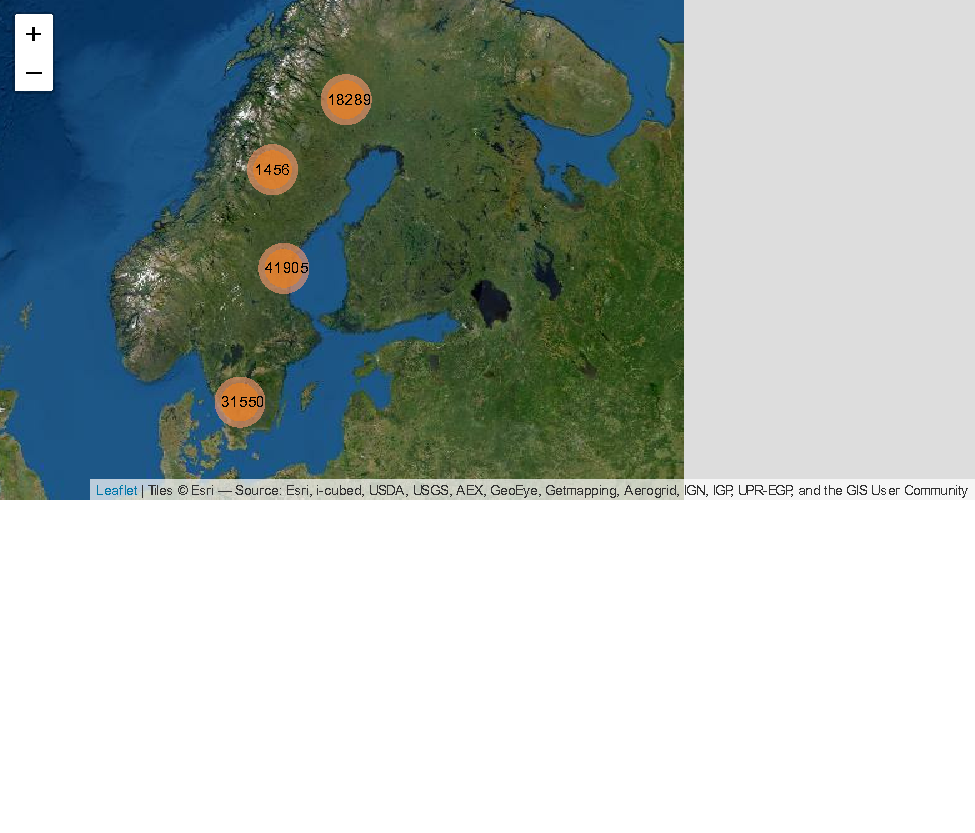
\includegraphics{r-tools-tutorial_files/figure-latex/leaflet-1.pdf}

\hypertarget{temporal-summary}{%
\subsection{Temporal summary}\label{temporal-summary}}

A quick summary over the years reveals a drop in number of records over time.

\begin{Shaded}
\begin{Highlighting}[]
\FunctionTok{table}\NormalTok{(xf}\SpecialCharTok{$}\NormalTok{data}\SpecialCharTok{$}\NormalTok{year)}
\end{Highlighting}
\end{Shaded}

\begin{verbatim}
## 
##  2008  2009  2010  2011  2012 
## 17757 19300 19643 16853 19647
\end{verbatim}

\begin{Shaded}
\begin{Highlighting}[]
\FunctionTok{hist}\NormalTok{(xf}\SpecialCharTok{$}\NormalTok{data}\SpecialCharTok{$}\NormalTok{year, }
     \AttributeTok{breaks =} \FunctionTok{seq}\NormalTok{(y1, y2), }
     \AttributeTok{xlab =} \StringTok{"Year"}\NormalTok{, }
     \AttributeTok{main =} \StringTok{""}\NormalTok{)}
\end{Highlighting}
\end{Shaded}

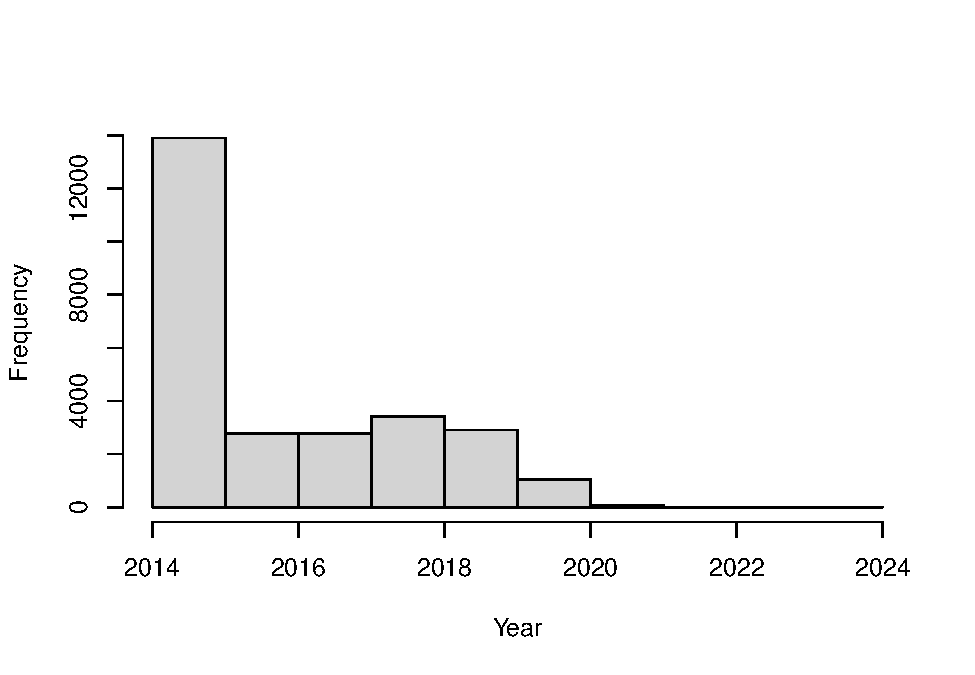
\includegraphics{r-tools-tutorial_files/figure-latex/timeHist-1.pdf}

\hypertarget{species-summary}{%
\subsection{Species summary}\label{species-summary}}

In the same way we can summarise the number of observations for each species, by common or scientific name.

\begin{Shaded}
\begin{Highlighting}[]
\NormalTok{sppTab }\OtherTok{\textless{}{-}} \FunctionTok{table}\NormalTok{(xf}\SpecialCharTok{$}\NormalTok{data}\SpecialCharTok{$}\NormalTok{commonName)}
\NormalTok{sppDF }\OtherTok{\textless{}{-}} \FunctionTok{as.data.frame}\NormalTok{(sppTab)}
\FunctionTok{colnames}\NormalTok{(sppDF)[}\DecValTok{1}\NormalTok{] }\OtherTok{\textless{}{-}} \StringTok{"species"}
\FunctionTok{head}\NormalTok{(sppDF)}
\end{Highlighting}
\end{Shaded}

\begin{verbatim}
##           species Freq
## 1                   61
## 2 Alpine bullhead 4615
## 3 American burbot 7081
## 4        Aral asp    6
## 5     Arctic char   46
## 6    aurora trout  856
\end{verbatim}

\begin{Shaded}
\begin{Highlighting}[]
\NormalTok{sppTab }\OtherTok{\textless{}{-}} \FunctionTok{table}\NormalTok{(xf}\SpecialCharTok{$}\NormalTok{data}\SpecialCharTok{$}\NormalTok{scientificName)}
\NormalTok{sppDF }\OtherTok{\textless{}{-}} \FunctionTok{as.data.frame}\NormalTok{(sppTab)}
\FunctionTok{colnames}\NormalTok{(sppDF)[}\DecValTok{1}\NormalTok{] }\OtherTok{\textless{}{-}} \StringTok{"species"}
\FunctionTok{head}\NormalTok{(sppDF)}
\end{Highlighting}
\end{Shaded}

\begin{verbatim}
##                                species Freq
## 1       Abramis brama (Linnaeus, 1758)   61
## 2   Alburnus alburnus (Linnaeus, 1758)  660
## 3   Anguilla anguilla (Linnaeus, 1758) 2140
## 4     Astacus astacus (Linnaeus, 1758)  618
## 5 Barbatula barbatula (Linnaeus, 1758)  620
## 6     Blicca bjoerkna (Linnaeus, 1758)   74
\end{verbatim}

Perhaps, you want to send this table as a .CSV file to a colleague. Save the table:

\begin{Shaded}
\begin{Highlighting}[]
\FunctionTok{write.csv}\NormalTok{(sppDF, }\StringTok{"SERS\_species\_summary.csv"}\NormalTok{)}
\CommentTok{\# }\AlertTok{NOTE}\CommentTok{: again this will be saved on your working directory}
\end{Highlighting}
\end{Shaded}

\hypertarget{spatial-biodiversity-analysis}{%
\subsection{Spatial biodiversity analysis}\label{spatial-biodiversity-analysis}}

Let's now ask: How does the species richness vary across Sweden?

For this we want to summarise occurrences species-wise over a defined grid instead of plotting every observation point. First we need to overlay the observations with a grid. Here we are using the standard Swedish grids with grid square size of 50, 25, 10 or 5 km provided as data in the SBDI4R package (with Coordinate Reference System = WGS84, EPSG:4326).

\begin{Shaded}
\begin{Highlighting}[]
\FunctionTok{library}\NormalTok{(sf) }\CommentTok{\# the function coordinates() and proj4string() are in sp}
\FunctionTok{library}\NormalTok{(rgeos) }\CommentTok{\# the function over() is in package rgeos}
\CommentTok{\# load some shapes over Sweden\textquotesingle{}s political borders}
\FunctionTok{data}\NormalTok{(}\StringTok{"swe\_wgs84"}\NormalTok{, }\AttributeTok{package =} \StringTok{"SBDI4R"}\NormalTok{, }\AttributeTok{envir =} \FunctionTok{environment}\NormalTok{())}
\CommentTok{\# a standard 50 km grid}
\FunctionTok{data}\NormalTok{(}\StringTok{"Sweden\_Grid\_50km\_Wgs84"}\NormalTok{, }\AttributeTok{package =} \StringTok{"SBDI4R"}\NormalTok{, }\AttributeTok{envir =} \FunctionTok{environment}\NormalTok{())}

\NormalTok{grid }\OtherTok{\textless{}{-}}\NormalTok{ Sweden\_Grid\_50km\_Wgs84}

\CommentTok{\# make the observations spatial}
\CommentTok{\# }\AlertTok{NOTE}\CommentTok{: make sure there are no NAs in the columns defining the coordinates}
\CommentTok{\# xf$data[!is.na(xf$data$longitude) | !is.na(xf$data$latitude),]}

\NormalTok{obs }\OtherTok{\textless{}{-}} \FunctionTok{st\_as\_sf}\NormalTok{(}\FunctionTok{as.data.frame}\NormalTok{(xf}\SpecialCharTok{$}\NormalTok{data),}
                \AttributeTok{coords =} \FunctionTok{c}\NormalTok{(}\StringTok{"longitude"}\NormalTok{,}\StringTok{"latitude"}\NormalTok{),}
                \AttributeTok{crs =} \FunctionTok{st\_crs}\NormalTok{(}\DecValTok{4326}\NormalTok{))}

\CommentTok{\# overlay the occurrence data with the grid}
\NormalTok{ObsInGridListID }\OtherTok{\textless{}{-}} \FunctionTok{st\_intersects}\NormalTok{(grid, obs)}
\NormalTok{ObsInGridList }\OtherTok{\textless{}{-}} \FunctionTok{lapply}\NormalTok{(ObsInGridListID, }\ControlFlowTok{function}\NormalTok{(x) }\FunctionTok{st\_drop\_geometry}\NormalTok{(obs[x,]))}
\NormalTok{wNonEmpty }\OtherTok{\textless{}{-}} \FunctionTok{unname}\NormalTok{( }\FunctionTok{which}\NormalTok{( }\FunctionTok{unlist}\NormalTok{(}\FunctionTok{lapply}\NormalTok{(ObsInGridList, nrow)) }\SpecialCharTok{!=} \DecValTok{0}\NormalTok{) )}
\end{Highlighting}
\end{Shaded}

The result \texttt{ObsInGridList} is a \texttt{list} object with a subset of the data for each grid cell. Now summarise occurrences within grid cells:

\begin{Shaded}
\begin{Highlighting}[]
\CommentTok{\# check n the total number of observations}
\FunctionTok{sum}\NormalTok{(}\FunctionTok{unlist}\NormalTok{(}\FunctionTok{lapply}\NormalTok{(ObsInGridList, nrow)))}
\end{Highlighting}
\end{Shaded}

\begin{verbatim}
## [1] 93200
\end{verbatim}

\begin{Shaded}
\begin{Highlighting}[]
\CommentTok{\# apply a summary over the grid cells }
\NormalTok{nCells }\OtherTok{\textless{}{-}} \FunctionTok{length}\NormalTok{(ObsInGridList)}
\NormalTok{res }\OtherTok{\textless{}{-}} \FunctionTok{data.frame}\NormalTok{(}\StringTok{"nObs"} \OtherTok{=} \FunctionTok{as.numeric}\NormalTok{(}\FunctionTok{rep}\NormalTok{(}\ConstantTok{NA}\NormalTok{,nCells)),}
                  \StringTok{"nYears"} \OtherTok{=} \FunctionTok{as.numeric}\NormalTok{(}\FunctionTok{rep}\NormalTok{(}\ConstantTok{NA}\NormalTok{,nCells)),}
                  \StringTok{"nSpp"} \OtherTok{=} \FunctionTok{as.numeric}\NormalTok{(}\FunctionTok{rep}\NormalTok{(}\ConstantTok{NA}\NormalTok{,nCells)),}
                  \AttributeTok{row.names =} \FunctionTok{row.names}\NormalTok{(grid),}
                  \AttributeTok{stringsAsFactors =} \ConstantTok{FALSE}\NormalTok{)}

\NormalTok{cols2use }\OtherTok{\textless{}{-}} \FunctionTok{c}\NormalTok{(}\StringTok{"scientificName"}\NormalTok{, }\StringTok{"year"}\NormalTok{)}
\NormalTok{dataRes }\OtherTok{\textless{}{-}} \FunctionTok{lapply}\NormalTok{(ObsInGridList[wNonEmpty], }
                  \ControlFlowTok{function}\NormalTok{(x)\{}
\NormalTok{                    x }\OtherTok{\textless{}{-}}\NormalTok{ x[,cols2use]}
                    \FunctionTok{colnames}\NormalTok{(x) }\OtherTok{\textless{}{-}} \FunctionTok{c}\NormalTok{(}\StringTok{"scientificName"}\NormalTok{, }\StringTok{"year"}\NormalTok{)}
                    \FunctionTok{return}\NormalTok{(}\FunctionTok{c}\NormalTok{(}\StringTok{"nObs"} \OtherTok{=} \FunctionTok{length}\NormalTok{(x[,}\StringTok{"scientificName"}\NormalTok{]),}
                             \StringTok{"nYears"} \OtherTok{=} \FunctionTok{length}\NormalTok{(}\FunctionTok{unique}\NormalTok{(x[,}\StringTok{"year"}\NormalTok{])),}
                             \StringTok{"nSpp"} \OtherTok{=} \FunctionTok{length}\NormalTok{(}\FunctionTok{unique}\NormalTok{(x[,}\StringTok{"scientificName"}\NormalTok{]))}
\NormalTok{                             )}
\NormalTok{                           )}
\NormalTok{                    \}}
\NormalTok{                  )}
\NormalTok{dataRes }\OtherTok{\textless{}{-}} \FunctionTok{as.data.frame}\NormalTok{(dplyr}\SpecialCharTok{::}\FunctionTok{bind\_rows}\NormalTok{(dataRes, }\AttributeTok{.id =} \StringTok{"gridID"}\NormalTok{))}
\NormalTok{res[wNonEmpty,] }\OtherTok{\textless{}{-}}\NormalTok{ dataRes[,}\SpecialCharTok{{-}}\DecValTok{1}\NormalTok{]}
\NormalTok{resSf }\OtherTok{\textless{}{-}} \FunctionTok{st\_as\_sf}\NormalTok{(}\FunctionTok{data.frame}\NormalTok{(res, }\FunctionTok{st\_geometry}\NormalTok{(grid)))}
\end{Highlighting}
\end{Shaded}

And finally plot the grid summary as a map:

\begin{Shaded}
\begin{Highlighting}[]
\NormalTok{palBW }\OtherTok{\textless{}{-}}\NormalTok{ leaflet}\SpecialCharTok{::}\FunctionTok{colorNumeric}\NormalTok{(}\FunctionTok{c}\NormalTok{(}\StringTok{"white"}\NormalTok{, }\StringTok{"navyblue"}\NormalTok{),}
                               \FunctionTok{c}\NormalTok{(}\DecValTok{0}\NormalTok{, }\FunctionTok{max}\NormalTok{(resSf}\SpecialCharTok{$}\NormalTok{nSpp, }\AttributeTok{na.rm =} \ConstantTok{TRUE}\NormalTok{)),}
                               \AttributeTok{na.color =} \StringTok{"transparent"}\NormalTok{)}
\NormalTok{oldpar }\OtherTok{\textless{}{-}} \FunctionTok{par}\NormalTok{()}
\FunctionTok{par}\NormalTok{(}\AttributeTok{mar =} \FunctionTok{c}\NormalTok{(}\DecValTok{1}\NormalTok{,}\DecValTok{1}\NormalTok{,}\DecValTok{0}\NormalTok{,}\DecValTok{0}\NormalTok{))}
\FunctionTok{plot}\NormalTok{(resSf}\SpecialCharTok{$}\NormalTok{geometry, }\AttributeTok{col =} \FunctionTok{palBW}\NormalTok{(resSf}\SpecialCharTok{$}\NormalTok{nSpp), }\AttributeTok{border =} \ConstantTok{NA}\NormalTok{)}
\FunctionTok{plot}\NormalTok{(swe\_wgs84}\SpecialCharTok{$}\NormalTok{Border}\SpecialCharTok{$}\NormalTok{geometry, }\AttributeTok{border =} \DecValTok{1}\NormalTok{, }\AttributeTok{lwd =} \DecValTok{1}\NormalTok{, }\AttributeTok{add =}\NormalTok{ T)}
\FunctionTok{legend}\NormalTok{(}\StringTok{"bottomleft"}\NormalTok{, }
       \AttributeTok{legend =} \FunctionTok{round}\NormalTok{(}\FunctionTok{seq}\NormalTok{(}\DecValTok{0}\NormalTok{, }\FunctionTok{max}\NormalTok{(resSf}\SpecialCharTok{$}\NormalTok{nSpp, }\AttributeTok{na.rm =} \ConstantTok{TRUE}\NormalTok{), }\AttributeTok{length.out =} \DecValTok{5}\NormalTok{)),}
       \AttributeTok{col =} \FunctionTok{palBW}\NormalTok{(}\FunctionTok{seq}\NormalTok{(}\DecValTok{0}\NormalTok{, }\FunctionTok{max}\NormalTok{(resSf}\SpecialCharTok{$}\NormalTok{nSpp, }\AttributeTok{na.rm =} \ConstantTok{TRUE}\NormalTok{), }\AttributeTok{length.out =} \DecValTok{5}\NormalTok{)),}
       \AttributeTok{title =} \StringTok{"Number of }\SpecialCharTok{\textbackslash{}n}\StringTok{species"}\NormalTok{, }\AttributeTok{pch =} \DecValTok{15}\NormalTok{, }\AttributeTok{bty=}\StringTok{"n"}\NormalTok{)}
\FunctionTok{par}\NormalTok{(oldpar)}
\end{Highlighting}
\end{Shaded}

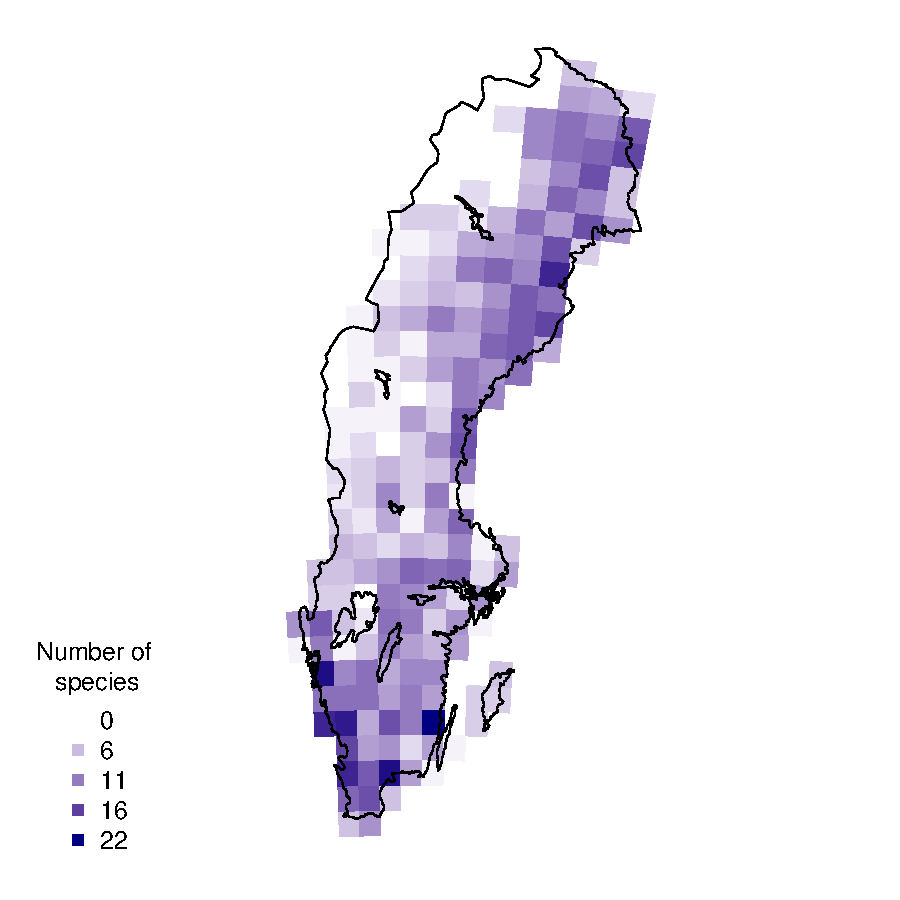
\includegraphics{r-tools-tutorial_files/figure-latex/gridPlot-1.pdf}

We may now ask whether species richness varies across latitude. So we go further by arranging the observations by latitude:

\begin{Shaded}
\begin{Highlighting}[]
\FunctionTok{library}\NormalTok{(dplyr)}
\FunctionTok{library}\NormalTok{(tidyr)}
\NormalTok{xgridded }\OtherTok{\textless{}{-}}\NormalTok{ xf}\SpecialCharTok{$}\NormalTok{data }\SpecialCharTok{\%\textgreater{}\%}
    \FunctionTok{mutate}\NormalTok{(}\AttributeTok{longitude =} \FunctionTok{round}\NormalTok{(longitude }\SpecialCharTok{*} \DecValTok{4}\NormalTok{)}\SpecialCharTok{/}\DecValTok{4}\NormalTok{, }
           \AttributeTok{latitude =} \FunctionTok{round}\NormalTok{(latitude }\SpecialCharTok{*} \DecValTok{4}\NormalTok{)}\SpecialCharTok{/}\DecValTok{4}\NormalTok{) }\SpecialCharTok{\%\textgreater{}\%}
    \FunctionTok{group\_by}\NormalTok{(longitude,latitude) }\SpecialCharTok{\%\textgreater{}\%}
    \DocumentationTok{\#\# subset to vars of interest}
    \FunctionTok{select}\NormalTok{(longitude, latitude, species) }\SpecialCharTok{\%\textgreater{}\%}
    \DocumentationTok{\#\# take one row per cell per species (presence)}
    \FunctionTok{distinct}\NormalTok{() }\SpecialCharTok{\%\textgreater{}\%}
    \DocumentationTok{\#\# calculate species richness}
    \FunctionTok{mutate}\NormalTok{(}\AttributeTok{richness =} \FunctionTok{n}\NormalTok{()) }\SpecialCharTok{\%\textgreater{}\%}
    \DocumentationTok{\#\# convert to wide format (sites by species)}
    \FunctionTok{mutate}\NormalTok{(}\AttributeTok{present =} \DecValTok{1}\NormalTok{) }\SpecialCharTok{\%\textgreater{}\%}
    \FunctionTok{do}\NormalTok{(tidyr}\SpecialCharTok{::}\FunctionTok{pivot\_wider}\NormalTok{(}\AttributeTok{data =}\NormalTok{ .,  }
                          \AttributeTok{names\_from =}\NormalTok{ species, }
                          \AttributeTok{values\_from =}\NormalTok{ present, }
                          \AttributeTok{values\_fill =} \DecValTok{0}\NormalTok{)) }\SpecialCharTok{\%\textgreater{}\%}
    \FunctionTok{ungroup}\NormalTok{()}
\DocumentationTok{\#\# where a species was not present, it will have NA: convert these to 0}
\NormalTok{sppcols }\OtherTok{\textless{}{-}} \FunctionTok{setdiff}\NormalTok{(}\FunctionTok{names}\NormalTok{(xgridded),}
                   \FunctionTok{c}\NormalTok{(}\StringTok{"longitude"}\NormalTok{, }\StringTok{"latitude"}\NormalTok{, }\StringTok{"richness"}\NormalTok{))}
\NormalTok{xgridded }\OtherTok{\textless{}{-}}\NormalTok{ xgridded }\SpecialCharTok{\%\textgreater{}\%} 
  \FunctionTok{mutate\_at}\NormalTok{(sppcols, }\ControlFlowTok{function}\NormalTok{(z) }\FunctionTok{ifelse}\NormalTok{(}\FunctionTok{is.na}\NormalTok{(z), }\DecValTok{0}\NormalTok{, z))}
\end{Highlighting}
\end{Shaded}

And plot it accordingly:

\begin{Shaded}
\begin{Highlighting}[]
\FunctionTok{library}\NormalTok{(ggplot2)}

\FunctionTok{ggplot}\NormalTok{(xgridded, }\FunctionTok{aes}\NormalTok{(latitude, richness)) }\SpecialCharTok{+} 
  \FunctionTok{labs}\NormalTok{(}\AttributeTok{x =} \StringTok{"Latitude (º)"}\NormalTok{, }
       \AttributeTok{y =} \StringTok{"Species richness"}\NormalTok{) }\SpecialCharTok{+}
  \FunctionTok{lims}\NormalTok{(}\AttributeTok{y =} \FunctionTok{c}\NormalTok{(}\DecValTok{0}\NormalTok{,}\DecValTok{20}\NormalTok{)) }\SpecialCharTok{+}
  \FunctionTok{geom\_point}\NormalTok{() }\SpecialCharTok{+} 
  \FunctionTok{theme\_bw}\NormalTok{()}
\end{Highlighting}
\end{Shaded}

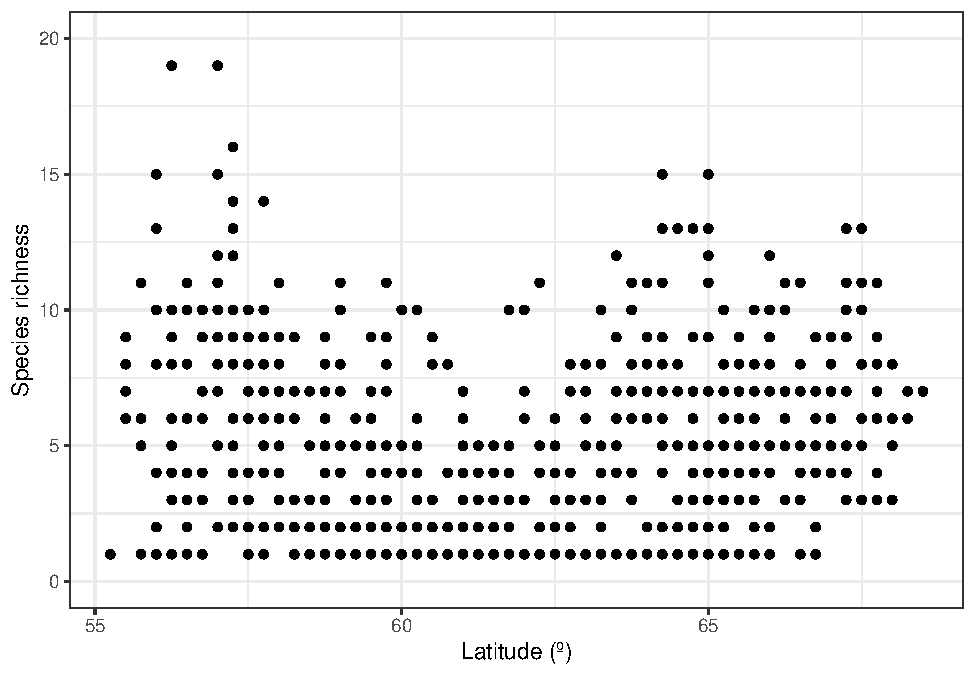
\includegraphics{r-tools-tutorial_files/figure-latex/plot_richLat-1.pdf}

\hypertarget{example-with-opportunistic-data-on-dragonflies}{%
\section{Example with opportunistic data on Dragonflies}\label{example-with-opportunistic-data-on-dragonflies}}

In this example we are interested in exploring opportunistically
collected data from the Swedish citizen science species observation
portal - Artportalen.

\hypertarget{name-searching}{%
\subsection{Name searching}\label{name-searching}}

To begin with, we want be sure there is an unequivocal way to find the
species within the order Odonata (dragonflies) and nothing else, so
let's search for ``odonata'':

\begin{Shaded}
\begin{Highlighting}[]
\NormalTok{sx }\OtherTok{\textless{}{-}} \FunctionTok{search\_fulltext}\NormalTok{(}\StringTok{"odonata"}\NormalTok{)}
\NormalTok{sx}\SpecialCharTok{$}\NormalTok{data[, }\FunctionTok{c}\NormalTok{(}\StringTok{"guid"}\NormalTok{, }\StringTok{"scientificName"}\NormalTok{, }\StringTok{"rank"}\NormalTok{, }\StringTok{"occurrenceCount"}\NormalTok{)]}
\end{Highlighting}
\end{Shaded}

\begin{verbatim}
## [1] "https://species.biodiversitydata.se/ws/search.json?q=odonata&fq=idxtype%3ATAXON"
\end{verbatim}

\begin{verbatim}
##       guid                          scientificName    rank occurrenceCount
## 1 10072832  Odonata associated gemycircularvirus 2 species               0
## 2  7367071    Ramalina fastigiata var. odonata Hue variety               0
## 3      789                                 Odonata   order           14121
## 4  8062407 Bdellodes odonata Wallace & Mahon, 1976 species               0
## 5  9829523  Odonata associated gemycircularvirus 1 species               0
\end{verbatim}

We quickly see there that other taxonomic levels appear too, and also
species that look suspiciously as not belonging to dragonflies. But
there is only one order. Let's refine the search. To know which search
fields we can use to filter the search we use the function
\texttt{sbdi\_fields(fields\_type\ =\ "general")}. The search field we are looking
for is ``order\_s''.

\begin{Shaded}
\begin{Highlighting}[]
\NormalTok{sx }\OtherTok{\textless{}{-}} \FunctionTok{search\_fulltext}\NormalTok{(}\AttributeTok{fq =} \StringTok{"order\_s:Odonata"}\NormalTok{, }\AttributeTok{page\_size =} \DecValTok{10}\NormalTok{)}
\NormalTok{sx}\SpecialCharTok{$}\NormalTok{data[, }\FunctionTok{c}\NormalTok{(}\StringTok{"scientificName"}\NormalTok{, }\StringTok{"rank"}\NormalTok{, }\StringTok{"occurrenceCount"}\NormalTok{)]}
\end{Highlighting}
\end{Shaded}

\begin{verbatim}
## [1] "https://species.biodiversitydata.se/ws/search.json?fq=order_s%3AOdonata&fq=idxtype%3ATAXON&pageSize=10"
\end{verbatim}

\begin{verbatim}
##        guid                        scientificName    rank occurrenceCount
## 1  11034676      Notoneura xanthe Lieftinck, 1938 species               0
## 2  11034731   Protoneura bifurcata Sjöstedt, 1918 species               0
## 3  11034937        Oxygomphus chapini Klots, 1944 species               0
## 4  11035128    Xerolestes pallidus (Rambur, 1842) species               0
## 5  11035335    Mesothemis mithroides Brauer, 1900 species               0
## 6  11029091 Paracercion luzonicum (Asahina, 1968) species               0
## 7  11029136         Onychargia stellata Ris, 1915 species               0
## 8  11029184         Nehalennia sophia Selys, 1840 species               0
## 9  11029206     Lestes lundquisti Lieftinck, 1949 species               0
## 10 11029310                Lestes concinnus Selys species               0
\end{verbatim}

Now we can download the taxonomic data (note that the search is
case-sensitive):

\begin{Shaded}
\begin{Highlighting}[]
\NormalTok{tx }\OtherTok{\textless{}{-}} \FunctionTok{taxinfo\_download}\NormalTok{(}\StringTok{"order\_s:Odonata"}\NormalTok{, }
                       \AttributeTok{fields =} \FunctionTok{c}\NormalTok{(}\StringTok{"guid"}\NormalTok{, }\StringTok{"order\_s"}\NormalTok{,}\StringTok{"genus\_s"}\NormalTok{, }\StringTok{"specificEpithet\_s"}\NormalTok{, }
                                  \StringTok{"scientificName"}\NormalTok{,  }\StringTok{"canonicalName\_s"}\NormalTok{, }\StringTok{"rank"}\NormalTok{), }
                       \AttributeTok{verbose =} \ConstantTok{FALSE}\NormalTok{)}
\NormalTok{tx }\OtherTok{\textless{}{-}}\NormalTok{ tx[tx}\SpecialCharTok{$}\NormalTok{rank }\SpecialCharTok{==} \StringTok{"species"} \SpecialCharTok{\&}\NormalTok{ tx}\SpecialCharTok{$}\NormalTok{genusS }\SpecialCharTok{!=} \StringTok{""}\NormalTok{,] }\DocumentationTok{\#\# restrict to species and not hybrids}
\end{Highlighting}
\end{Shaded}

You can save the \texttt{tx} object as the complete species list for later use.

\hypertarget{filter-the-search-to-get-the-observations}{%
\subsection{Filter the search to get the observations}\label{filter-the-search-to-get-the-observations}}

We start by searching for the data resource we are interested in using
the function \texttt{pick\_filter()}. This is an interactive query guiding you
through the many resources available to filtering your query (data
resources, spatial layers, and curated species lists).

\begin{Shaded}
\begin{Highlighting}[]
\CommentTok{\# follow the instructions }
\NormalTok{fq\_str }\OtherTok{\textless{}{-}} \FunctionTok{pick\_filter}\NormalTok{(}\StringTok{"resource"}\NormalTok{) }
\end{Highlighting}
\end{Shaded}

Follow the instructions. Your choices here would have been ``in3'' --\textgreater{}
``dr5''. Your variable \texttt{fq\_str} will now contain a string
``data\_resource\_uid:dr5''.

We only want to look at data from year 2000 to 2010:

\begin{Shaded}
\begin{Highlighting}[]
\NormalTok{y1 }\OtherTok{\textless{}{-}} \DecValTok{2000}
\NormalTok{y2 }\OtherTok{\textless{}{-}} \DecValTok{2010}
\NormalTok{fq\_str }\OtherTok{\textless{}{-}} \FunctionTok{c}\NormalTok{(fq\_str, }\FunctionTok{paste0}\NormalTok{(}\StringTok{"year:["}\NormalTok{, y1, }\StringTok{" TO "}\NormalTok{, y2,}\StringTok{"]"}\NormalTok{))}
\CommentTok{\# Note the square brackets are hard limits}
\end{Highlighting}
\end{Shaded}

We also want to filter spatially for Southern Sweden
(\href{https://en.wikipedia.org/wiki/G\%C3\%B6taland}{Götaland}).

Vector spatial layers (eg. polygons) can be imported in a number of
different ways. SBDI APIs take as search input polygons in the so-called
WKT \href{https://www.geoapi.org/3.0/javadoc/org/opengis/referencing/doc-files/WKT.html}{Well Known
Text}
format. So the first step is to load a vector layer and transform it
into a WKT string. You could instead use the data we provid in the
SBDI4R package \texttt{data("swe")}.

\begin{Shaded}
\begin{Highlighting}[]
\FunctionTok{data}\NormalTok{(}\StringTok{"swe"}\NormalTok{,}\AttributeTok{package =} \StringTok{"SBDI4R"}\NormalTok{)}
\NormalTok{wGotaland }\OtherTok{\textless{}{-}}\NormalTok{ swe}\SpecialCharTok{$}\NormalTok{Counties}\SpecialCharTok{$}\NormalTok{LnNamn }\SpecialCharTok{\%in\%} \FunctionTok{c}\NormalTok{(}\StringTok{"Blekinge"}\NormalTok{, }\StringTok{"Gotlands"}\NormalTok{, }\StringTok{"Hallands"}\NormalTok{, }
                                        \StringTok{"Jönköpings"}\NormalTok{, }\StringTok{"Kalmar"}\NormalTok{, }\StringTok{"Kronobergs"}\NormalTok{, }
                                        \StringTok{"Östergötlands"}\NormalTok{, }\StringTok{"Skåne"}\NormalTok{, }\StringTok{"Västra Götalands"}\NormalTok{)}
\NormalTok{gotaland\_c }\OtherTok{\textless{}{-}}\NormalTok{ swe}\SpecialCharTok{$}\NormalTok{Counties[wGotaland,]}
\end{Highlighting}
\end{Shaded}

There are details about this polygon that we need to take care before.
The WKT string should not be too long to be accepted by the API service.
Also, the polygon we just got is projected in the coordinate system
SWEREF99 TM, and the API service only accepts coordinates in a geodesic
coordinate system WGS84. Let's construct the WKT string:

\begin{Shaded}
\begin{Highlighting}[]
\CommentTok{\# transform the CRS}
\NormalTok{gotaland\_c }\OtherTok{\textless{}{-}} \FunctionTok{st\_transform}\NormalTok{(gotaland\_c,}
                           \AttributeTok{crs =} \FunctionTok{st\_crs}\NormalTok{(}\DecValTok{4326}\NormalTok{))}

\CommentTok{\# disolve the counties into one polygon}
\NormalTok{gotaland }\OtherTok{\textless{}{-}} \FunctionTok{st\_union}\NormalTok{(gotaland\_c)}

\CommentTok{\# create a convex hull of the polygon to simplify the geometry and }
\CommentTok{\# reduce the length of the WKT string}
\NormalTok{gotaland\_ch }\OtherTok{\textless{}{-}} \FunctionTok{st\_convex\_hull}\NormalTok{(gotaland)}

\CommentTok{\# cast it as MULTIPOLYGON as this is what SBDIs API need}
\CommentTok{\# }\AlertTok{NOTE}\CommentTok{: as of today, the SBDI APIs will only work properly if the polygon is }
\CommentTok{\# submitted as a MULTIPOLYGON}
\NormalTok{gotaland\_ch }\OtherTok{\textless{}{-}} \FunctionTok{st\_cast}\NormalTok{(gotaland\_ch, }\AttributeTok{to =} \StringTok{"MULTIPOLYGON"}\NormalTok{)}

\CommentTok{\# create WKT string}
\NormalTok{wkt }\OtherTok{\textless{}{-}} \FunctionTok{st\_as\_text}\NormalTok{(gotaland\_ch)}
\end{Highlighting}
\end{Shaded}

The WKT string then looks like this:

\begin{verbatim}
## [1] "MULTIPOLYGON (((13.33575 55.34003, 12.81633 55.38594, 11.25342 58.35786, 11.13161 58.90942, 11.13145 59.01184, 11.21142 59.0897, 11.31566 59.11651, 11.82032 59.23553, 11.94833 59.26237, 12.06197 59.27159, 12.23104 59.27357, 15.79383 59.03876, 15.84306 59.02498, 19.2889 57.99043, 19.3058 57.96888, 18.90037 57.44014, 18.86704 57.39753, 18.3725 57.00678, 18.30044 56.9528, 16.40805 56.20229, 14.19057 55.38557, 13.33575 55.34003)))"
\end{verbatim}

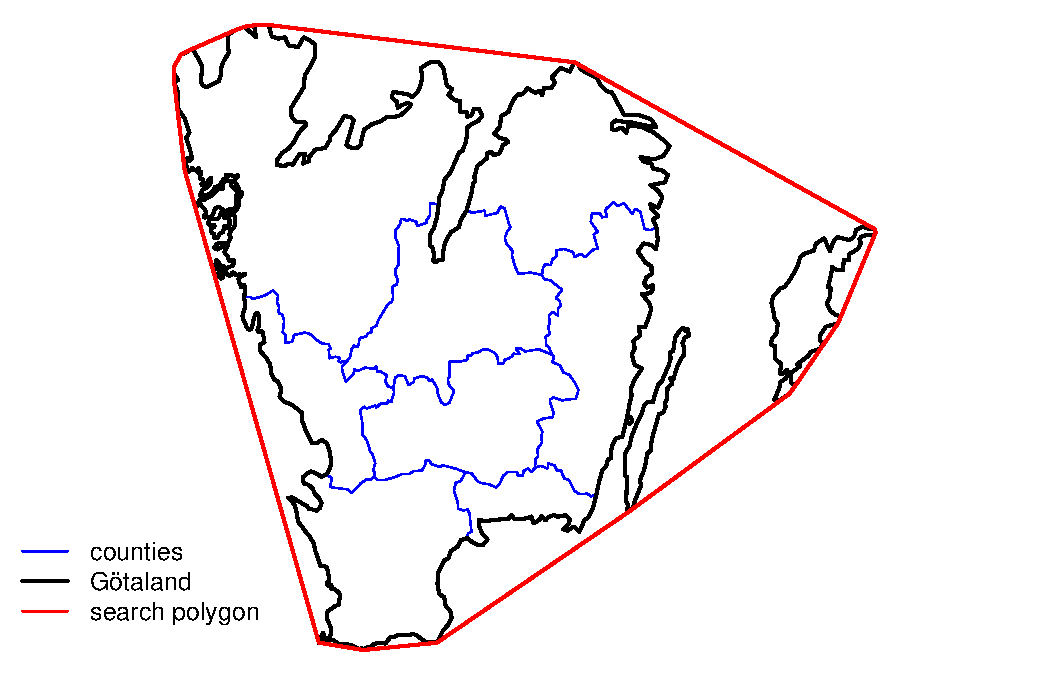
\includegraphics{r-tools-tutorial_files/figure-latex/searchpoly-1.pdf}

Next, we download the observations using the command \texttt{occurrences()},
but be aware that the search fields may not be the same as those used to
search for taxa. We therefore recommend using the function
\texttt{sbdi\_fields("occurrence")} to find out which search fields we can use
to filter for occurrences. Here we see that the field we need this time
is ``order''.

\begin{Shaded}
\begin{Highlighting}[]
\NormalTok{xf }\OtherTok{\textless{}{-}} \FunctionTok{occurrences}\NormalTok{(}\AttributeTok{taxon =} \StringTok{"order:Odonata"}\NormalTok{, }
                  \AttributeTok{fq =}\NormalTok{ fq\_str,}
                  \AttributeTok{wkt =}\NormalTok{ wkt,}
                  \AttributeTok{extra =} \StringTok{"collector"}\NormalTok{,}
                  \AttributeTok{email =} \StringTok{"sbdi4r{-}test@biodiversitydata.se"}\NormalTok{, }
                  \AttributeTok{download\_reason\_id =} \DecValTok{10}\NormalTok{)}
\end{Highlighting}
\end{Shaded}

We have now downloaded the data locally and depending on your
configuration this will be cached on your computer. However, as the
search and download could take long time, we recommend to save the data
locally. appropriate

\begin{Shaded}
\begin{Highlighting}[]
\FunctionTok{save}\NormalTok{(xf, }\AttributeTok{file =} \StringTok{"an\_appropriate\_name.rdata"}\NormalTok{)}
\FunctionTok{load}\NormalTok{(}\AttributeTok{file =} \StringTok{"an\_appropriate\_name.rdata"}\NormalTok{)}
\end{Highlighting}
\end{Shaded}

\hypertarget{quality-and-fit-for-use-check}{%
\subsection{Quality and fit-for-use check}\label{quality-and-fit-for-use-check}}

Before we can use the observation records we need to know if the
observation effort (sampling effort) has varied over time and in space.
We can approximate observation effort from the data by defining field
visits i.e.~occasions at which an observer has sampled observations. We
reconstruct field visits (that is, assign each observation a visitUID)
using using the package \href{https://greensway.github.io/BIRDS/}{BIRDS}.
Additionally we want the data to be summarized over a grid of 25 km
(provided through the SBDI4R package). The following functions will
perform many different summaries at the same time. Please refer to the
BIRDS package documentation for more detail.

\begin{Shaded}
\begin{Highlighting}[]
\NormalTok{remotes}\SpecialCharTok{::}\FunctionTok{install\_github}\NormalTok{(}\StringTok{"Greensway/BIRDS"}\NormalTok{)}
\end{Highlighting}
\end{Shaded}

\begin{verbatim}
## xfun        (0.24   -> 0.26  ) [CRAN]
## digest      (0.6.27 -> 0.6.28) [CRAN]
## stringi     (1.7.4  -> 1.7.5 ) [CRAN]
## mime        (0.11   -> 0.12  ) [CRAN]
## tibble      (3.1.3  -> 3.1.5 ) [CRAN]
## matrixStats (0.59.0 -> 0.61.0) [CRAN]
## e1071       (1.7-7  -> 1.7-9 ) [CRAN]
## robustbase  (0.93-8 -> 0.93-9) [CRAN]
## tidyr       (1.1.3  -> 1.1.4 ) [CRAN]
## rgdal       (1.5-23 -> 1.5-27) [CRAN]
## 
##   There are binary versions available but the source versions are later:
##         binary source needs_compilation
## stringi  1.7.4  1.7.5              TRUE
## tibble   3.1.4  3.1.5              TRUE
## 
## package 'xfun' successfully unpacked and MD5 sums checked
## package 'digest' successfully unpacked and MD5 sums checked
## package 'mime' successfully unpacked and MD5 sums checked
## package 'matrixStats' successfully unpacked and MD5 sums checked
## package 'e1071' successfully unpacked and MD5 sums checked
## package 'robustbase' successfully unpacked and MD5 sums checked
## package 'rgdal' successfully unpacked and MD5 sums checked
## 
## The downloaded binary packages are in
##  C:\Users\Alejandro\AppData\Local\Temp\Rtmpw5RsYS\downloaded_packages
##          checking for file 'C:\Users\Alejandro\AppData\Local\Temp\Rtmpw5RsYS\remotes5020a394a91\Greensway-BIRDS-8a336fd/DESCRIPTION' ...     checking for file 'C:\Users\Alejandro\AppData\Local\Temp\Rtmpw5RsYS\remotes5020a394a91\Greensway-BIRDS-8a336fd/DESCRIPTION' ...   v  checking for file 'C:\Users\Alejandro\AppData\Local\Temp\Rtmpw5RsYS\remotes5020a394a91\Greensway-BIRDS-8a336fd/DESCRIPTION'
##       -  preparing 'BIRDS': (1.7s)
##    checking DESCRIPTION meta-information ...     checking DESCRIPTION meta-information ...   v  checking DESCRIPTION meta-information
##       -  installing the package to process help pages
##       -  saving partial Rd database (13.6s)
##       -  checking for LF line-endings in source and make files and shell scripts
##       -  checking for empty or unneeded directories
##   Removed empty directory      Removed empty directory 'BIRDS/data-raw'
##       -  building 'BIRDS_0.2.2.tar.gz'
##      
## 
\end{verbatim}

\begin{Shaded}
\begin{Highlighting}[]
\FunctionTok{library}\NormalTok{(BIRDS)}
\end{Highlighting}
\end{Shaded}

\begin{Shaded}
\begin{Highlighting}[]
\NormalTok{OB }\OtherTok{\textless{}{-}} \FunctionTok{organiseBirds}\NormalTok{(xf}\SpecialCharTok{$}\NormalTok{data, }\AttributeTok{sppCol =} \StringTok{"species"}\NormalTok{ , }
                    \CommentTok{\# We only want observations identified at the species level}
                    \AttributeTok{taxonRankCol =} \StringTok{"rank"}\NormalTok{, }\AttributeTok{taxonRank =} \StringTok{"species"}\NormalTok{, }
                    \CommentTok{\# the visits are defined by collector and named locality}
                    \AttributeTok{idCols =} \FunctionTok{c}\NormalTok{(}\StringTok{"locality"}\NormalTok{, }\StringTok{"collector"}\NormalTok{), }
                    \AttributeTok{timeCols =} \FunctionTok{c}\NormalTok{(}\StringTok{"year"}\NormalTok{, }\StringTok{"month"}\NormalTok{, }\StringTok{"day"}\NormalTok{), }
                    \AttributeTok{xyCols =} \FunctionTok{c}\NormalTok{(}\StringTok{"longitude"}\NormalTok{,}\StringTok{"latitude"}\NormalTok{) )}

\CommentTok{\# We don\textquotesingle{}t need the whole grid, just the piece that overlaps our searching polygon}
\NormalTok{wInt }\OtherTok{\textless{}{-}} \FunctionTok{unlist}\NormalTok{(}\FunctionTok{st\_intersects}\NormalTok{(gotaland, Sweden\_Grid\_25km\_Wgs84))}
\NormalTok{gotaland\_grid25 }\OtherTok{\textless{}{-}}\NormalTok{ Sweden\_Grid\_25km\_Wgs84[wInt,]}

\NormalTok{SB }\OtherTok{\textless{}{-}} \FunctionTok{summariseBirds}\NormalTok{(OB, }\AttributeTok{grid =}\NormalTok{ gotaland\_grid25, }\AttributeTok{spillOver =} \StringTok{"unique"}\NormalTok{)}
\end{Highlighting}
\end{Shaded}

Once summarised, we can see over space and for a few selected years how
the number of observations is distributed:

\begin{Shaded}
\begin{Highlighting}[]
\NormalTok{maxC }\OtherTok{\textless{}{-}} \FunctionTok{max}\NormalTok{(SB}\SpecialCharTok{$}\NormalTok{spatial}\SpecialCharTok{$}\NormalTok{nObs, }\AttributeTok{na.rm =} \ConstantTok{TRUE}\NormalTok{)}
\NormalTok{palBW }\OtherTok{\textless{}{-}}\NormalTok{ leaflet}\SpecialCharTok{::}\FunctionTok{colorNumeric}\NormalTok{(}\FunctionTok{c}\NormalTok{(}\StringTok{"white"}\NormalTok{, }\StringTok{"navyblue"}\NormalTok{), }
                               \FunctionTok{c}\NormalTok{(}\DecValTok{0}\NormalTok{, maxC), }
                               \AttributeTok{na.color =} \StringTok{"transparent"}\NormalTok{)}
\NormalTok{oldpar }\OtherTok{\textless{}{-}} \FunctionTok{par}\NormalTok{()}
\FunctionTok{par}\NormalTok{(}\AttributeTok{mar =} \FunctionTok{c}\NormalTok{(}\DecValTok{1}\NormalTok{,}\DecValTok{1}\NormalTok{,}\DecValTok{1}\NormalTok{,}\DecValTok{1}\NormalTok{), }\AttributeTok{mfrow=}\FunctionTok{c}\NormalTok{(}\DecValTok{1}\NormalTok{,}\DecValTok{3}\NormalTok{))}
\FunctionTok{plot}\NormalTok{(SB}\SpecialCharTok{$}\NormalTok{spatial}\SpecialCharTok{$}\NormalTok{geometry, }\AttributeTok{col=}\FunctionTok{palBW}\NormalTok{(SB}\SpecialCharTok{$}\NormalTok{spatial}\SpecialCharTok{$}\NormalTok{nObs),}
     \AttributeTok{border =} \StringTok{"grey"}\NormalTok{, }\AttributeTok{main=}\StringTok{"All years"}\NormalTok{) }\DocumentationTok{\#\# with palette}
\FunctionTok{legend}\NormalTok{(}\StringTok{"bottomleft"}\NormalTok{, }\AttributeTok{inset =} \FunctionTok{c}\NormalTok{(}\DecValTok{0}\NormalTok{,}\FloatTok{0.05}\NormalTok{),}
       \AttributeTok{legend =} \FunctionTok{round}\NormalTok{(}\FunctionTok{seq}\NormalTok{(}\DecValTok{0}\NormalTok{, maxC, }\AttributeTok{length.out =} \DecValTok{5}\NormalTok{)),}
       \AttributeTok{col =} \FunctionTok{palBW}\NormalTok{(}\FunctionTok{seq}\NormalTok{(}\DecValTok{0}\NormalTok{, maxC, }\AttributeTok{length.out =} \DecValTok{5}\NormalTok{)),}
       \AttributeTok{title =} \StringTok{"Number of }\SpecialCharTok{\textbackslash{}n}\StringTok{observations"}\NormalTok{, }\AttributeTok{pch =} \DecValTok{15}\NormalTok{, }\AttributeTok{bty=}\StringTok{"n"}\NormalTok{)}

\DocumentationTok{\#\# or export other combinations, e.g. one map per observed year}
\NormalTok{yearlySp }\OtherTok{\textless{}{-}} \FunctionTok{exportBirds}\NormalTok{(SB, }
                        \AttributeTok{dimension =} \StringTok{"spatial"}\NormalTok{, }
                        \AttributeTok{timeRes =} \StringTok{"yearly"}\NormalTok{, }
                        \AttributeTok{variable =} \StringTok{"nObs"}\NormalTok{, }
                        \AttributeTok{method =} \StringTok{"sum"}\NormalTok{)}

\NormalTok{maxC }\OtherTok{\textless{}{-}} \FunctionTok{max}\NormalTok{(yearlySp}\SpecialCharTok{$}\StringTok{\textquotesingle{}2005\textquotesingle{}}\NormalTok{, }\AttributeTok{na.rm =} \ConstantTok{TRUE}\NormalTok{)}
\NormalTok{palBW }\OtherTok{\textless{}{-}}\NormalTok{ leaflet}\SpecialCharTok{::}\FunctionTok{colorNumeric}\NormalTok{(}\FunctionTok{c}\NormalTok{(}\StringTok{"white"}\NormalTok{, }\StringTok{"navyblue"}\NormalTok{), }
                               \FunctionTok{c}\NormalTok{(}\DecValTok{0}\NormalTok{, maxC), }
                               \AttributeTok{na.color =} \StringTok{"transparent"}\NormalTok{)}

\FunctionTok{plot}\NormalTok{(yearlySp}\SpecialCharTok{$}\NormalTok{geometry, }\AttributeTok{col=}\FunctionTok{palBW}\NormalTok{(yearlySp}\SpecialCharTok{$}\StringTok{\textquotesingle{}2005\textquotesingle{}}\NormalTok{), }
     \AttributeTok{border =} \StringTok{"grey"}\NormalTok{,}\AttributeTok{main=}\StringTok{"2005"}\NormalTok{)}
\FunctionTok{legend}\NormalTok{(}\StringTok{"bottomleft"}\NormalTok{, }\AttributeTok{inset =} \FunctionTok{c}\NormalTok{(}\DecValTok{0}\NormalTok{,}\FloatTok{0.05}\NormalTok{),}
       \AttributeTok{legend =} \FunctionTok{round}\NormalTok{(}\FunctionTok{seq}\NormalTok{(}\DecValTok{0}\NormalTok{, maxC, }\AttributeTok{length.out =} \DecValTok{5}\NormalTok{)),}
       \AttributeTok{col =} \FunctionTok{palBW}\NormalTok{(}\FunctionTok{seq}\NormalTok{(}\DecValTok{0}\NormalTok{, maxC, }\AttributeTok{length.out =} \DecValTok{5}\NormalTok{)),}
       \AttributeTok{border =} \StringTok{"grey"}\NormalTok{,}
       \AttributeTok{title =} \StringTok{"Number of }\SpecialCharTok{\textbackslash{}n}\StringTok{observations"}\NormalTok{, }\AttributeTok{pch =} \DecValTok{15}\NormalTok{, }\AttributeTok{bty=}\StringTok{"n"}\NormalTok{)}

\NormalTok{maxC }\OtherTok{\textless{}{-}} \FunctionTok{max}\NormalTok{(yearlySp}\StringTok{\textquotesingle{}2010\textquotesingle{}}\NormalTok{, }\AttributeTok{na.rm =} \ConstantTok{TRUE}\NormalTok{)}
\NormalTok{palBW }\OtherTok{\textless{}{-}}\NormalTok{ leaflet}\SpecialCharTok{::}\FunctionTok{colorNumeric}\NormalTok{(}\FunctionTok{c}\NormalTok{(}\StringTok{"white"}\NormalTok{, }\StringTok{"navyblue"}\NormalTok{), }
                               \FunctionTok{c}\NormalTok{(}\DecValTok{0}\NormalTok{, maxC), }
                               \AttributeTok{na.color =} \StringTok{"transparent"}\NormalTok{)}

\FunctionTok{plot}\NormalTok{(yearlySp}\SpecialCharTok{$}\NormalTok{geometry, }\AttributeTok{col=}\FunctionTok{palBW}\NormalTok{(yearlySp}\SpecialCharTok{$}\StringTok{\textquotesingle{}2010\textquotesingle{}}\NormalTok{), }
     \AttributeTok{border =} \StringTok{"grey"}\NormalTok{,}\AttributeTok{main=}\StringTok{"2010"}\NormalTok{)}
\FunctionTok{legend}\NormalTok{(}\StringTok{"bottomleft"}\NormalTok{, }\AttributeTok{inset =} \FunctionTok{c}\NormalTok{(}\DecValTok{0}\NormalTok{,}\FloatTok{0.05}\NormalTok{),}
       \AttributeTok{legend =} \FunctionTok{round}\NormalTok{(}\FunctionTok{seq}\NormalTok{(}\DecValTok{0}\NormalTok{, maxC, }\AttributeTok{length.out =} \DecValTok{5}\NormalTok{)),}
       \AttributeTok{col =} \FunctionTok{palBW}\NormalTok{(}\FunctionTok{seq}\NormalTok{(}\DecValTok{0}\NormalTok{, maxC, }\AttributeTok{length.out =} \DecValTok{5}\NormalTok{)),}
       \AttributeTok{border =} \StringTok{"grey"}\NormalTok{,}
       \AttributeTok{title =} \StringTok{"Number of }\SpecialCharTok{\textbackslash{}n}\StringTok{observations"}\NormalTok{, }\AttributeTok{pch =} \DecValTok{15}\NormalTok{, }\AttributeTok{bty=}\StringTok{"n"}\NormalTok{)}
\FunctionTok{par}\NormalTok{(oldpar)}
\end{Highlighting}
\end{Shaded}

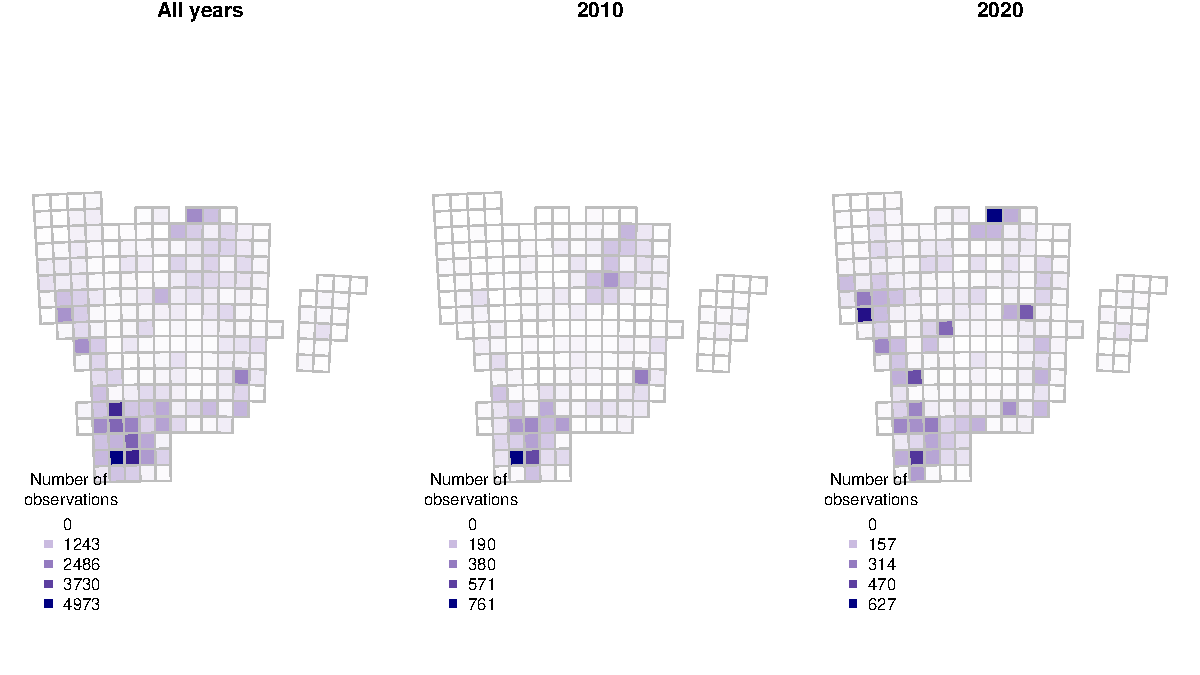
\includegraphics{r-tools-tutorial_files/figure-latex/plotBIRDSspatial-1.pdf}

We now want to use the number of field visits as the measure for
sampling effort. :

\begin{Shaded}
\begin{Highlighting}[]
\FunctionTok{library}\NormalTok{(cowplot)}
\FunctionTok{library}\NormalTok{(ggplot2)}
\FunctionTok{library}\NormalTok{(colorRamps)}
\FunctionTok{library}\NormalTok{(gridExtra)}

\NormalTok{vis }\OtherTok{\textless{}{-}} \FunctionTok{ggplot}\NormalTok{(}\AttributeTok{data =}\NormalTok{ SB}\SpecialCharTok{$}\NormalTok{spatial, }\FunctionTok{aes}\NormalTok{( }\AttributeTok{fill =}\NormalTok{ nVis)) }\SpecialCharTok{+}
  \FunctionTok{geom\_sf}\NormalTok{() }\SpecialCharTok{+}
  \FunctionTok{ggtitle}\NormalTok{(}\StringTok{"Visits"}\NormalTok{) }\SpecialCharTok{+}
  \FunctionTok{scale\_fill\_gradient}\NormalTok{(}\AttributeTok{low =} \StringTok{"\#56B1F7"}\NormalTok{,}
                      \AttributeTok{high =} \StringTok{"\#132B43"}\NormalTok{,}
                      \AttributeTok{na.value =} \ConstantTok{NA}\NormalTok{) }\SpecialCharTok{+}
  \FunctionTok{theme}\NormalTok{(}\AttributeTok{plot.margin =} \FunctionTok{margin}\NormalTok{(}\DecValTok{1}\NormalTok{, }\DecValTok{1}\NormalTok{, }\DecValTok{1}\NormalTok{, }\DecValTok{1}\NormalTok{, }\StringTok{"pt"}\NormalTok{)) }\SpecialCharTok{+}
  \FunctionTok{theme\_cowplot}\NormalTok{()}

\NormalTok{spp }\OtherTok{\textless{}{-}} \FunctionTok{ggplot}\NormalTok{(}\AttributeTok{data =}\NormalTok{ SB}\SpecialCharTok{$}\NormalTok{spatial, }\FunctionTok{aes}\NormalTok{( }\AttributeTok{fill =}\NormalTok{ nSpp)) }\SpecialCharTok{+}
  \FunctionTok{geom\_sf}\NormalTok{() }\SpecialCharTok{+}
  \FunctionTok{ggtitle}\NormalTok{(}\StringTok{"Number of species"}\NormalTok{) }\SpecialCharTok{+}
  \FunctionTok{scale\_fill\_gradient}\NormalTok{(}\AttributeTok{low =} \StringTok{"\#56B1F7"}\NormalTok{,}
                      \AttributeTok{high =} \StringTok{"\#132B43"}\NormalTok{,}
                      \AttributeTok{na.value =} \ConstantTok{NA}\NormalTok{) }\SpecialCharTok{+}
  \FunctionTok{theme}\NormalTok{(}\AttributeTok{plot.margin =} \FunctionTok{margin}\NormalTok{(}\DecValTok{1}\NormalTok{, }\DecValTok{1}\NormalTok{, }\DecValTok{1}\NormalTok{, }\DecValTok{1}\NormalTok{, }\StringTok{"pt"}\NormalTok{)) }\SpecialCharTok{+}
  \FunctionTok{theme\_cowplot}\NormalTok{()}

\FunctionTok{grid.arrange}\NormalTok{(vis, spp, }\AttributeTok{ncol =} \DecValTok{2}\NormalTok{)}
\end{Highlighting}
\end{Shaded}

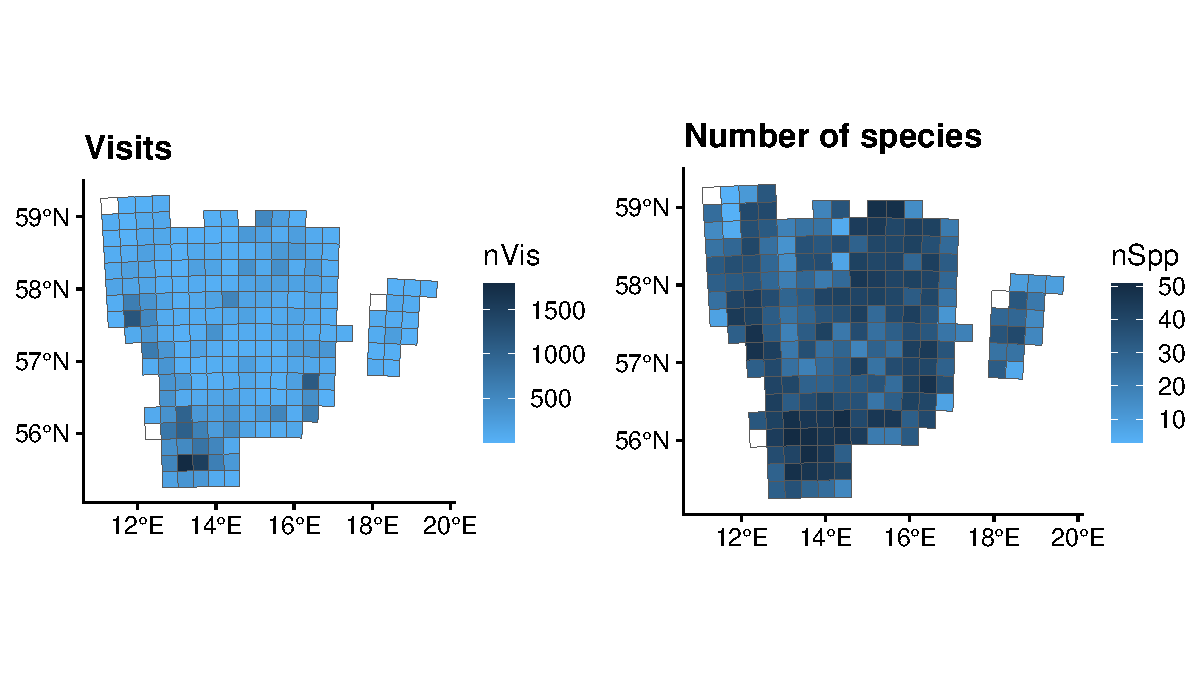
\includegraphics{r-tools-tutorial_files/figure-latex/ggplot1-1.pdf}

\hypertarget{temporal-check}{%
\paragraph{Temporal check}\label{temporal-check}}

We see that \texttt{SB} contains an element called \texttt{SB\$temporal} that contains
a daily time series with time-specific rows when there is information.
\texttt{xts} also supports day time, but dating below day resolution is not yet
implemented in the \texttt{BIRDS} package.

\begin{Shaded}
\begin{Highlighting}[]
\NormalTok{sb.xts }\OtherTok{\textless{}{-}}\NormalTok{ SB}\SpecialCharTok{$}\NormalTok{temporal}
\FunctionTok{head}\NormalTok{(sb.xts, }\DecValTok{5}\NormalTok{)}
\end{Highlighting}
\end{Shaded}

\begin{verbatim}
##            nObs nVis nSpp
## 2000-03-24    1    1    1
## 2000-04-05    4    3    3
## 2000-04-06   11    6    3
## 2000-04-10    1    1    1
## 2000-04-12    3    3    1
\end{verbatim}

Sub-setting is convenient in \texttt{xts} as you can do it with its dates and
with a \texttt{/} for a range of dates.

\begin{Shaded}
\begin{Highlighting}[]
\NormalTok{sb.xts[}\StringTok{"2010{-}09{-}07"}\NormalTok{] }\CommentTok{\#a specific day}
\end{Highlighting}
\end{Shaded}

\begin{verbatim}
##            nObs nVis nSpp
## 2010-09-07   19   10   12
\end{verbatim}

\begin{Shaded}
\begin{Highlighting}[]
\NormalTok{sb.xts[}\StringTok{"2010{-}09{-}01/2010{-}09{-}15"}\NormalTok{] }\CommentTok{\#for a period}
\end{Highlighting}
\end{Shaded}

\begin{verbatim}
##            nObs nVis nSpp
## 2010-09-01   46   19   14
## 2010-09-02   28   14   12
## 2010-09-03   23   10   10
## 2010-09-04   64   20   18
## 2010-09-05   74   27   12
## 2010-09-06   18    5   11
## 2010-09-07   19   10   12
## 2010-09-08   13    6    8
## 2010-09-09   32   12   14
## 2010-09-10    1    1    1
## 2010-09-11   16    9    8
## 2010-09-12   20   10    8
## 2010-09-13   14    5    9
## 2010-09-14    1    1    1
## 2010-09-15    3    3    2
\end{verbatim}

\begin{Shaded}
\begin{Highlighting}[]
\NormalTok{sb.xts[}\StringTok{"2010{-}09"}\NormalTok{] }\CommentTok{\#a specific month}
\end{Highlighting}
\end{Shaded}

\begin{verbatim}
##            nObs nVis nSpp
## 2010-09-01   46   19   14
## 2010-09-02   28   14   12
## 2010-09-03   23   10   10
## 2010-09-04   64   20   18
## 2010-09-05   74   27   12
## 2010-09-06   18    5   11
## 2010-09-07   19   10   12
## 2010-09-08   13    6    8
## 2010-09-09   32   12   14
## 2010-09-10    1    1    1
## 2010-09-11   16    9    8
## 2010-09-12   20   10    8
## 2010-09-13   14    5    9
## 2010-09-14    1    1    1
## 2010-09-15    3    3    2
## 2010-09-17    3    2    3
## 2010-09-18    9    5    5
## 2010-09-19   12    7    5
## 2010-09-21    3    2    3
## 2010-09-22    4    4    2
## 2010-09-23    3    3    2
## 2010-09-24   10    5    5
## 2010-09-25    7    4    6
## 2010-09-26    7    6    2
## 2010-09-28    2    2    2
## 2010-09-29    5    3    4
## 2010-09-30    2    2    2
\end{verbatim}

The package \texttt{xts} has several tools for converting to different time
periods. Here we use \texttt{apply.monthly} to obtain the total number of
observations and visits per month. The plot command for an object of
calss \texttt{xts} provides a many features. This makes it fairly easy to
customize your plots. Read more in \texttt{?plot.xts}.

\begin{Shaded}
\begin{Highlighting}[]
\FunctionTok{library}\NormalTok{(xts)}
\NormalTok{obs.m }\OtherTok{\textless{}{-}} \FunctionTok{apply.monthly}\NormalTok{(sb.xts}\SpecialCharTok{$}\NormalTok{nObs, }\StringTok{"sum"}\NormalTok{, }\AttributeTok{na.rm =} \ConstantTok{TRUE}\NormalTok{)}
\NormalTok{vis.m }\OtherTok{\textless{}{-}} \FunctionTok{apply.monthly}\NormalTok{(sb.xts}\SpecialCharTok{$}\NormalTok{nVis, }\StringTok{"sum"}\NormalTok{, }\AttributeTok{na.rm =} \ConstantTok{TRUE}\NormalTok{)}

\FunctionTok{plot}\NormalTok{(obs.m, }
     \AttributeTok{col =} \StringTok{"darkblue"}\NormalTok{, }
     \AttributeTok{grid.ticks.on =} \StringTok{"month"}\NormalTok{, }
     \AttributeTok{major.ticks =} \StringTok{"year"}\NormalTok{, }
     \AttributeTok{grid.col =} \StringTok{"lightgrey"}\NormalTok{,  }
     \AttributeTok{main =} \StringTok{"Total number of daily observations and visits per month"}\NormalTok{)}

\FunctionTok{lines}\NormalTok{(vis.m, }\AttributeTok{col =} \StringTok{"orange"}\NormalTok{, }\AttributeTok{lwd =} \DecValTok{2}\NormalTok{, }\AttributeTok{on =} \DecValTok{1}\NormalTok{)}
\end{Highlighting}
\end{Shaded}

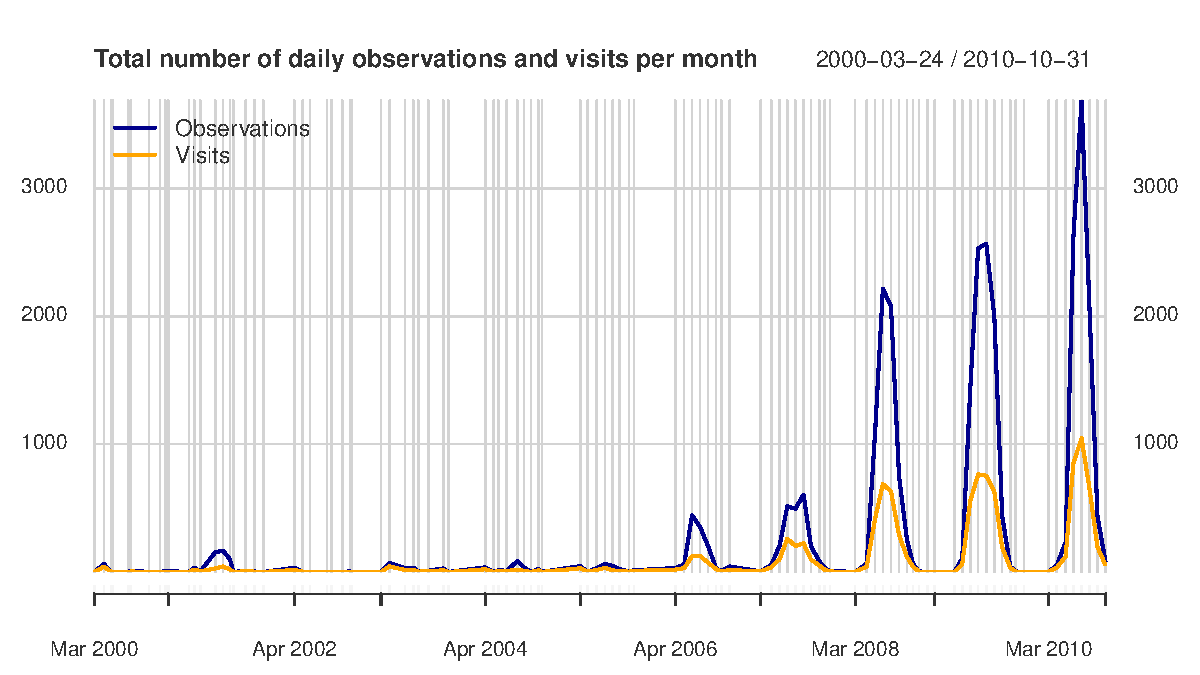
\includegraphics{r-tools-tutorial_files/figure-latex/unnamed-chunk-15-1.pdf}

\hypertarget{species-trends}{%
\subsection{Species trends}\label{species-trends}}

We can now look at some particular species and ask whether those have
changed in occurrence over time:

\begin{Shaded}
\begin{Highlighting}[]
\FunctionTok{speciesSummary}\NormalTok{(SB)[,}\DecValTok{1}\SpecialCharTok{:}\DecValTok{4}\NormalTok{]}
\end{Highlighting}
\end{Shaded}

\begin{verbatim}
##                       species nCells nObs nVis
## 1              Aeshna affinis      3   32   27
## 2             Aeshna caerulea      6   13   13
## 3               Aeshna cyanea    128  896  861
## 4              Aeshna grandis    156 1765 1735
## 5             Aeshna isoceles     25  172  169
## 6               Aeshna juncea    101  366  353
## 7                Aeshna mixta     81  677  646
## 8              Aeshna serrata     13   39   38
## 9           Aeshna subarctica     35  108   99
## 10             Aeshna viridis     13   40   35
## 11             Anax imperator     51  559  515
## 12            Anax parthenope      2    5    5
## 13        Brachytron pratense     93  505  492
## 14       Calopteryx splendens    102  682  628
## 15           Calopteryx virgo    124 1061 1007
## 16         Coenagrion armatum     23   74   67
## 17      Coenagrion hastulatum    118  941  908
## 18      Coenagrion johanssoni     15   75   70
## 19       Coenagrion lunulatum     42  111  104
## 20          Coenagrion puella    124 1415 1360
## 21      Coenagrion pulchellum    124 1439 1392
## 22     Cordulegaster boltonii     75  500  493
## 23             Cordulia aenea    122 1072 1053
## 24      Enallagma cyathigerum    149 1717 1630
## 25        Epitheca bimaculata     16   36   35
## 26           Erythromma najas     97  774  741
## 27       Erythromma viridulum     13  143  126
## 28      Gomphus vulgatissimus     48  160  155
## 29           Ischnura elegans    124 1351 1294
## 30           Ischnura pumilio     22  110   95
## 31               Lestes dryas     52  214  206
## 32              Lestes sponsa    147 1454 1385
## 33              Lestes virens     50  201  188
## 34     Leucorrhinia albifrons     47  185  180
## 35      Leucorrhinia caudalis     34  143  136
## 36         Leucorrhinia dubia     85  338  320
## 37    Leucorrhinia pectoralis     85  368  351
## 38     Leucorrhinia rubicunda     96  445  432
## 39         Libellula depressa    110  569  546
## 40            Libellula fulva      9  101   90
## 41   Libellula quadrimaculata    160 2096 2047
## 42        Nehalennia speciosa      3   34   33
## 43   Onychogomphus forcipatus     76  447  445
## 44      Orthetrum cancellatum    129 1079 1025
## 45     Orthetrum coerulescens     76  253  246
## 46       Platycnemis pennipes     92  545  529
## 47        Pyrrhosoma nymphula    127  974  945
## 48       Somatochlora arctica     28   45   42
## 49 Somatochlora flavomaculata     90  427  420
## 50     Somatochlora metallica    109  621  612
## 51             Sympecma fusca     50  269  264
## 52          Sympecma paedisca      2    5    5
## 53            Sympetrum danae    136  803  768
## 54        Sympetrum flaveolum     82  302  295
## 55     Sympetrum fonscolombii      2    2    2
## 56       Sympetrum sanguineum    137 1268 1224
## 57       Sympetrum striolatum     84  311  298
## 58         Sympetrum vulgatum    128 1072 1016
\end{verbatim}

We pick two species and compare their trends in number of visits where
the species where reported, relative to the total number of visits.

\begin{Shaded}
\begin{Highlighting}[]
\FunctionTok{library}\NormalTok{(dplyr)}
\NormalTok{sppCount }\OtherTok{\textless{}{-}} \FunctionTok{obsData}\NormalTok{(OB) }\SpecialCharTok{|}\ErrorTok{\textgreater{}} 
    \FunctionTok{group\_by}\NormalTok{(year, visitUID) }\SpecialCharTok{|}\ErrorTok{\textgreater{}} 
    \FunctionTok{summarise}\NormalTok{(}\StringTok{"focalCountLq"} \OtherTok{=} \FunctionTok{sum}\NormalTok{(scientificName }\SpecialCharTok{==} \StringTok{"Libellula quadrimaculata"}\NormalTok{),}
              \StringTok{"focalCountSd"} \OtherTok{=} \FunctionTok{sum}\NormalTok{(scientificName }\SpecialCharTok{==} \StringTok{"Sympetrum sanguineum"}\NormalTok{),}
              \StringTok{"sppLength"} \OtherTok{=} \FunctionTok{length}\NormalTok{(}\FunctionTok{unique}\NormalTok{(scientificName)), }
              \AttributeTok{.groups =} \StringTok{"drop"}\NormalTok{) }\SpecialCharTok{|}\ErrorTok{\textgreater{}} 
    \FunctionTok{ungroup}\NormalTok{() }\SpecialCharTok{|}\ErrorTok{\textgreater{}} 
    \FunctionTok{group\_by}\NormalTok{(year) }\SpecialCharTok{|}\ErrorTok{\textgreater{}} 
    \FunctionTok{summarise}\NormalTok{(}\StringTok{"focalCountLq"} \OtherTok{=} \FunctionTok{sum}\NormalTok{(focalCountLq),}
              \StringTok{"focalCountSd"} \OtherTok{=} \FunctionTok{sum}\NormalTok{(focalCountSd),}
              \StringTok{"nVis"} \OtherTok{=} \FunctionTok{length}\NormalTok{(}\FunctionTok{unique}\NormalTok{(visitUID)),}
              \StringTok{"relCountLq"} \OtherTok{=}\NormalTok{ focalCountLq }\SpecialCharTok{/}\NormalTok{ nVis,}
              \StringTok{"relCountSd"} \OtherTok{=}\NormalTok{ focalCountSd }\SpecialCharTok{/}\NormalTok{ nVis,}
              \AttributeTok{.groups =} \ConstantTok{NULL}\NormalTok{)}

\NormalTok{oldpar }\OtherTok{\textless{}{-}} \FunctionTok{par}\NormalTok{(}\AttributeTok{no.readonly =} \ConstantTok{TRUE}\NormalTok{)}
\FunctionTok{plot}\NormalTok{(sppCount}\SpecialCharTok{$}\NormalTok{year, sppCount}\SpecialCharTok{$}\NormalTok{relCountLq, }
     \AttributeTok{type =} \StringTok{"l"}\NormalTok{, }\AttributeTok{lwd =} \DecValTok{3}\NormalTok{, }\AttributeTok{xlab =} \StringTok{"Year"}\NormalTok{, }
     \AttributeTok{ylab =} \StringTok{"Relative number of visits with observations"}\NormalTok{, }
     \AttributeTok{ylim =} \FunctionTok{c}\NormalTok{(}\DecValTok{0}\NormalTok{, }\FunctionTok{max}\NormalTok{(sppCount}\SpecialCharTok{$}\NormalTok{relCountLq)), }
     \AttributeTok{xaxp =} \FunctionTok{c}\NormalTok{(}\DecValTok{2000}\NormalTok{, }\DecValTok{2010}\NormalTok{, }\DecValTok{10}\NormalTok{))}
\FunctionTok{lines}\NormalTok{(sppCount}\SpecialCharTok{$}\NormalTok{year, sppCount}\SpecialCharTok{$}\NormalTok{relCountSd, }\AttributeTok{lwd =} \DecValTok{3}\NormalTok{, }\AttributeTok{col =} \StringTok{"\#78D2EB"}\NormalTok{)}
\FunctionTok{legend}\NormalTok{(}\StringTok{"bottomright"}\NormalTok{, }
       \AttributeTok{legend =} \FunctionTok{c}\NormalTok{(}\StringTok{"Libellula quadrimaculata"}\NormalTok{,}\StringTok{"Sympetrum sanguineum"}\NormalTok{), }
       \AttributeTok{text.font =} \DecValTok{3}\NormalTok{, }\AttributeTok{col =} \FunctionTok{c}\NormalTok{(}\StringTok{"black"}\NormalTok{, }\StringTok{"\#78D2EB"}\NormalTok{), }\AttributeTok{lwd =} \DecValTok{3}\NormalTok{, }\AttributeTok{bty =} \StringTok{"n"}\NormalTok{)}
\end{Highlighting}
\end{Shaded}

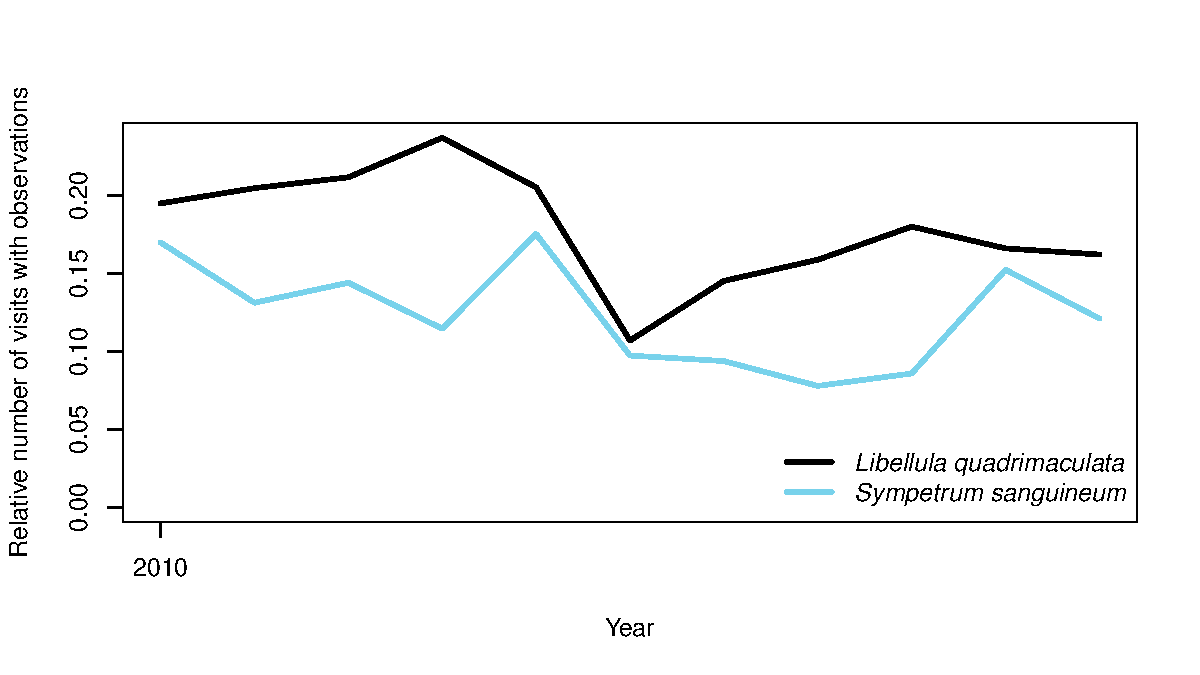
\includegraphics{r-tools-tutorial_files/figure-latex/trends-1.pdf}

\begin{Shaded}
\begin{Highlighting}[]
\FunctionTok{par}\NormalTok{(oldpar)}
\end{Highlighting}
\end{Shaded}


  \bibliography{references.bib}

\end{document}
